% Generated by Sphinx.
\def\sphinxdocclass{report}
\documentclass[letterpaper,12pt,english]{sphinxmanual}
\usepackage[utf8]{inputenc}
\DeclareUnicodeCharacter{00A0}{\nobreakspace}
\usepackage{cmap}
\usepackage[T1]{fontenc}
\usepackage{babel}
\usepackage{times}
\usepackage[Bjarne]{fncychap}
\usepackage{longtable}
\usepackage{sphinx}
\usepackage{multirow}

        \usepackage{times}
    

\title{Scrapple Documentation}
\date{March 31, 2015}
\release{}
\author{Alex Mathew, Harish Balakrishnan}
\newcommand{\sphinxlogo}{}
\renewcommand{\releasename}{}
\makeindex

\makeatletter
\def\PYG@reset{\let\PYG@it=\relax \let\PYG@bf=\relax%
    \let\PYG@ul=\relax \let\PYG@tc=\relax%
    \let\PYG@bc=\relax \let\PYG@ff=\relax}
\def\PYG@tok#1{\csname PYG@tok@#1\endcsname}
\def\PYG@toks#1+{\ifx\relax#1\empty\else%
    \PYG@tok{#1}\expandafter\PYG@toks\fi}
\def\PYG@do#1{\PYG@bc{\PYG@tc{\PYG@ul{%
    \PYG@it{\PYG@bf{\PYG@ff{#1}}}}}}}
\def\PYG#1#2{\PYG@reset\PYG@toks#1+\relax+\PYG@do{#2}}

\expandafter\def\csname PYG@tok@gd\endcsname{\def\PYG@tc##1{\textcolor[rgb]{0.63,0.00,0.00}{##1}}}
\expandafter\def\csname PYG@tok@gu\endcsname{\let\PYG@bf=\textbf\def\PYG@tc##1{\textcolor[rgb]{0.50,0.00,0.50}{##1}}}
\expandafter\def\csname PYG@tok@gt\endcsname{\def\PYG@tc##1{\textcolor[rgb]{0.00,0.27,0.87}{##1}}}
\expandafter\def\csname PYG@tok@gs\endcsname{\let\PYG@bf=\textbf}
\expandafter\def\csname PYG@tok@gr\endcsname{\def\PYG@tc##1{\textcolor[rgb]{1.00,0.00,0.00}{##1}}}
\expandafter\def\csname PYG@tok@cm\endcsname{\let\PYG@it=\textit\def\PYG@tc##1{\textcolor[rgb]{0.25,0.50,0.56}{##1}}}
\expandafter\def\csname PYG@tok@vg\endcsname{\def\PYG@tc##1{\textcolor[rgb]{0.73,0.38,0.84}{##1}}}
\expandafter\def\csname PYG@tok@m\endcsname{\def\PYG@tc##1{\textcolor[rgb]{0.13,0.50,0.31}{##1}}}
\expandafter\def\csname PYG@tok@mh\endcsname{\def\PYG@tc##1{\textcolor[rgb]{0.13,0.50,0.31}{##1}}}
\expandafter\def\csname PYG@tok@cs\endcsname{\def\PYG@tc##1{\textcolor[rgb]{0.25,0.50,0.56}{##1}}\def\PYG@bc##1{\setlength{\fboxsep}{0pt}\colorbox[rgb]{1.00,0.94,0.94}{\strut ##1}}}
\expandafter\def\csname PYG@tok@ge\endcsname{\let\PYG@it=\textit}
\expandafter\def\csname PYG@tok@vc\endcsname{\def\PYG@tc##1{\textcolor[rgb]{0.73,0.38,0.84}{##1}}}
\expandafter\def\csname PYG@tok@il\endcsname{\def\PYG@tc##1{\textcolor[rgb]{0.13,0.50,0.31}{##1}}}
\expandafter\def\csname PYG@tok@go\endcsname{\def\PYG@tc##1{\textcolor[rgb]{0.20,0.20,0.20}{##1}}}
\expandafter\def\csname PYG@tok@cp\endcsname{\def\PYG@tc##1{\textcolor[rgb]{0.00,0.44,0.13}{##1}}}
\expandafter\def\csname PYG@tok@gi\endcsname{\def\PYG@tc##1{\textcolor[rgb]{0.00,0.63,0.00}{##1}}}
\expandafter\def\csname PYG@tok@gh\endcsname{\let\PYG@bf=\textbf\def\PYG@tc##1{\textcolor[rgb]{0.00,0.00,0.50}{##1}}}
\expandafter\def\csname PYG@tok@ni\endcsname{\let\PYG@bf=\textbf\def\PYG@tc##1{\textcolor[rgb]{0.84,0.33,0.22}{##1}}}
\expandafter\def\csname PYG@tok@nl\endcsname{\let\PYG@bf=\textbf\def\PYG@tc##1{\textcolor[rgb]{0.00,0.13,0.44}{##1}}}
\expandafter\def\csname PYG@tok@nn\endcsname{\let\PYG@bf=\textbf\def\PYG@tc##1{\textcolor[rgb]{0.05,0.52,0.71}{##1}}}
\expandafter\def\csname PYG@tok@no\endcsname{\def\PYG@tc##1{\textcolor[rgb]{0.38,0.68,0.84}{##1}}}
\expandafter\def\csname PYG@tok@na\endcsname{\def\PYG@tc##1{\textcolor[rgb]{0.25,0.44,0.63}{##1}}}
\expandafter\def\csname PYG@tok@nb\endcsname{\def\PYG@tc##1{\textcolor[rgb]{0.00,0.44,0.13}{##1}}}
\expandafter\def\csname PYG@tok@nc\endcsname{\let\PYG@bf=\textbf\def\PYG@tc##1{\textcolor[rgb]{0.05,0.52,0.71}{##1}}}
\expandafter\def\csname PYG@tok@nd\endcsname{\let\PYG@bf=\textbf\def\PYG@tc##1{\textcolor[rgb]{0.33,0.33,0.33}{##1}}}
\expandafter\def\csname PYG@tok@ne\endcsname{\def\PYG@tc##1{\textcolor[rgb]{0.00,0.44,0.13}{##1}}}
\expandafter\def\csname PYG@tok@nf\endcsname{\def\PYG@tc##1{\textcolor[rgb]{0.02,0.16,0.49}{##1}}}
\expandafter\def\csname PYG@tok@si\endcsname{\let\PYG@it=\textit\def\PYG@tc##1{\textcolor[rgb]{0.44,0.63,0.82}{##1}}}
\expandafter\def\csname PYG@tok@s2\endcsname{\def\PYG@tc##1{\textcolor[rgb]{0.25,0.44,0.63}{##1}}}
\expandafter\def\csname PYG@tok@vi\endcsname{\def\PYG@tc##1{\textcolor[rgb]{0.73,0.38,0.84}{##1}}}
\expandafter\def\csname PYG@tok@nt\endcsname{\let\PYG@bf=\textbf\def\PYG@tc##1{\textcolor[rgb]{0.02,0.16,0.45}{##1}}}
\expandafter\def\csname PYG@tok@nv\endcsname{\def\PYG@tc##1{\textcolor[rgb]{0.73,0.38,0.84}{##1}}}
\expandafter\def\csname PYG@tok@s1\endcsname{\def\PYG@tc##1{\textcolor[rgb]{0.25,0.44,0.63}{##1}}}
\expandafter\def\csname PYG@tok@gp\endcsname{\let\PYG@bf=\textbf\def\PYG@tc##1{\textcolor[rgb]{0.78,0.36,0.04}{##1}}}
\expandafter\def\csname PYG@tok@sh\endcsname{\def\PYG@tc##1{\textcolor[rgb]{0.25,0.44,0.63}{##1}}}
\expandafter\def\csname PYG@tok@ow\endcsname{\let\PYG@bf=\textbf\def\PYG@tc##1{\textcolor[rgb]{0.00,0.44,0.13}{##1}}}
\expandafter\def\csname PYG@tok@sx\endcsname{\def\PYG@tc##1{\textcolor[rgb]{0.78,0.36,0.04}{##1}}}
\expandafter\def\csname PYG@tok@bp\endcsname{\def\PYG@tc##1{\textcolor[rgb]{0.00,0.44,0.13}{##1}}}
\expandafter\def\csname PYG@tok@c1\endcsname{\let\PYG@it=\textit\def\PYG@tc##1{\textcolor[rgb]{0.25,0.50,0.56}{##1}}}
\expandafter\def\csname PYG@tok@kc\endcsname{\let\PYG@bf=\textbf\def\PYG@tc##1{\textcolor[rgb]{0.00,0.44,0.13}{##1}}}
\expandafter\def\csname PYG@tok@c\endcsname{\let\PYG@it=\textit\def\PYG@tc##1{\textcolor[rgb]{0.25,0.50,0.56}{##1}}}
\expandafter\def\csname PYG@tok@mf\endcsname{\def\PYG@tc##1{\textcolor[rgb]{0.13,0.50,0.31}{##1}}}
\expandafter\def\csname PYG@tok@err\endcsname{\def\PYG@bc##1{\setlength{\fboxsep}{0pt}\fcolorbox[rgb]{1.00,0.00,0.00}{1,1,1}{\strut ##1}}}
\expandafter\def\csname PYG@tok@kd\endcsname{\let\PYG@bf=\textbf\def\PYG@tc##1{\textcolor[rgb]{0.00,0.44,0.13}{##1}}}
\expandafter\def\csname PYG@tok@ss\endcsname{\def\PYG@tc##1{\textcolor[rgb]{0.32,0.47,0.09}{##1}}}
\expandafter\def\csname PYG@tok@sr\endcsname{\def\PYG@tc##1{\textcolor[rgb]{0.14,0.33,0.53}{##1}}}
\expandafter\def\csname PYG@tok@mo\endcsname{\def\PYG@tc##1{\textcolor[rgb]{0.13,0.50,0.31}{##1}}}
\expandafter\def\csname PYG@tok@mi\endcsname{\def\PYG@tc##1{\textcolor[rgb]{0.13,0.50,0.31}{##1}}}
\expandafter\def\csname PYG@tok@kn\endcsname{\let\PYG@bf=\textbf\def\PYG@tc##1{\textcolor[rgb]{0.00,0.44,0.13}{##1}}}
\expandafter\def\csname PYG@tok@o\endcsname{\def\PYG@tc##1{\textcolor[rgb]{0.40,0.40,0.40}{##1}}}
\expandafter\def\csname PYG@tok@kr\endcsname{\let\PYG@bf=\textbf\def\PYG@tc##1{\textcolor[rgb]{0.00,0.44,0.13}{##1}}}
\expandafter\def\csname PYG@tok@s\endcsname{\def\PYG@tc##1{\textcolor[rgb]{0.25,0.44,0.63}{##1}}}
\expandafter\def\csname PYG@tok@kp\endcsname{\def\PYG@tc##1{\textcolor[rgb]{0.00,0.44,0.13}{##1}}}
\expandafter\def\csname PYG@tok@w\endcsname{\def\PYG@tc##1{\textcolor[rgb]{0.73,0.73,0.73}{##1}}}
\expandafter\def\csname PYG@tok@kt\endcsname{\def\PYG@tc##1{\textcolor[rgb]{0.56,0.13,0.00}{##1}}}
\expandafter\def\csname PYG@tok@sc\endcsname{\def\PYG@tc##1{\textcolor[rgb]{0.25,0.44,0.63}{##1}}}
\expandafter\def\csname PYG@tok@sb\endcsname{\def\PYG@tc##1{\textcolor[rgb]{0.25,0.44,0.63}{##1}}}
\expandafter\def\csname PYG@tok@k\endcsname{\let\PYG@bf=\textbf\def\PYG@tc##1{\textcolor[rgb]{0.00,0.44,0.13}{##1}}}
\expandafter\def\csname PYG@tok@se\endcsname{\let\PYG@bf=\textbf\def\PYG@tc##1{\textcolor[rgb]{0.25,0.44,0.63}{##1}}}
\expandafter\def\csname PYG@tok@sd\endcsname{\let\PYG@it=\textit\def\PYG@tc##1{\textcolor[rgb]{0.25,0.44,0.63}{##1}}}

\def\PYGZbs{\char`\\}
\def\PYGZus{\char`\_}
\def\PYGZob{\char`\{}
\def\PYGZcb{\char`\}}
\def\PYGZca{\char`\^}
\def\PYGZam{\char`\&}
\def\PYGZlt{\char`\<}
\def\PYGZgt{\char`\>}
\def\PYGZsh{\char`\#}
\def\PYGZpc{\char`\%}
\def\PYGZdl{\char`\$}
\def\PYGZhy{\char`\-}
\def\PYGZsq{\char`\'}
\def\PYGZdq{\char`\"}
\def\PYGZti{\char`\~}
% for compatibility with earlier versions
\def\PYGZat{@}
\def\PYGZlb{[}
\def\PYGZrb{]}
\makeatother

\renewcommand\PYGZsq{\textquotesingle}

\begin{document}

\maketitle
\tableofcontents
\phantomsection\label{index::doc}



\chapter{Synopsis}
\label{index:scrapple-version-documentation}\label{index:synopsis}
The Internet is a huge source of information. Several people may use data from the Internet to perform various activities, like research or analysis. Data extraction is a primary step involved in data mining and analysis. Extracting content from structured web pages is a vital task to be performed when the Internet is the principal source of data.

The current standards in web structure involve the use of CSS selectors or XPath expressions to select particular tags from which information can be extracted. Web pages are structured as element trees which can be parsed to traverse through the tags. This tree structure, which represents tags as parent/children/siblings, is very useful when tags should be represented in terms of the rest of the web page structure.

Scrapple is a project aimed at designing a framework for building web content extractors. Scrapple uses key-value based configuration files to define parameters to be considered in generating the extractor. It considers the base page URL, selectors for the data to be extracted, and the selector for the links to be crawled through. At its core, Scrapple abstracts the implementation of the extractor, focussing more on representing the selectors for the required tags. Scrapple can be used to generate single page content extractors or link crawlers.

This documentation contains information about how to use Scrapple and how Scrapple works.


\chapter{Introduction}
\label{index:introduction}
The Internet is a huge source of information. Several people may use data from the Internet to perform various activities, like research or analysis. However, there are two primary issues involved with using data from the Internet :
\begin{itemize}
\item {} 
You may not have any way to get information from a particular website, i.e, it may not provide an API for accessing the data.

\item {} 
Even if an API is provided, it may not give all the data needed. It is possible that there may be some data that is present on the web interface, but not provided through the API.

\end{itemize}

This is where web scrapers and web crawlers come in.


\section{Web scrapers \& web crawlers}
\label{index:web-scrapers-web-crawlers}
\textbf{Web scrapers}, also called \textbf{extractors}, are used to extract content from any particular page. They may use CSS Selectors or XPath expressions to point to a particular tag on the HTML structure of the page, and extract the content from that tag. The content extracted could be text from \code{\textless{}div\textgreater{}} tags, links from \code{\textless{}a\textgreater{}} tags, and so on.

\textbf{Web crawlers} are scripts that go through multiple links from a single base page. Given a base URL, it uses this page as an index page to many different pages. It goes through each of these pages, extracting the required content along the way.

Scrapers and crawlers can be written to extract necessary content from any page that you would need information from.


\section{Objective}
\label{index:objective}
Scrapple helps to reduce the hassle in manually writing the scripts needed to extract the required content. It involves the use of a configuration file that specifies property-value pairs of various parameters involved in constructing the required script.

The configuration file is a JSON document, consisting of the required key-value pairs. The user specifies the base URL of the page to work on, and also the tags of the data to be extracted. The user has a choice between CSS selectors and XPath expressions for specifying the target tags. Once the target tags have been specified, the other parameters are filled and the configuration file is completed. This configuration file is used by Scrapple to generate the required script and the execution is performed to generate the output of the scraper as a CSV/JSON document (depending on the argument passed while running the script). Thus, the user can obtain data they need without having extensive programming expertise to manually write the scripts required.


\section{The inspiration behind Scrapple}
\label{index:the-inspiration-behind-scrapple}
Scrapple is based on the best ideas involved in two projects :
\begin{itemize}
\item {} 
{\color{red}\bfseries{}{}`Scrapy{}`\_} : An application framework for crawling web sites and extracting structured data.

\item {} 
\href{http://dl.acm.org/citation.cfm?id=2628244}{Ducky} : A semi-automatic Web Wrapper to extract data according to the pre-defined and simple data extraction rule in the configuration file.

\end{itemize}


\chapter{Project timeline}
\label{index:project-timeline}\label{index:ducky}
The overall project work can be summarized in this Gantt chart.
\begin{figure}[htbp]
\centering
\capstart

\includegraphics{gantt.png}
\caption{Gantt chart - Project timeline}\end{figure}

The project repository was hosted on \href{http://github.com/}{GitHub}. This provided multiple benefits :
\begin{itemize}
\item {} 
Ease of collaboration between project members

\item {} 
Convenient version control of project

\item {} 
Setting up continuous integration testing on the project

\item {} 
Metrics for analysis of project progress

\end{itemize}

The metrics provided by GitHub can be used to visually represent the contributions to the project over the duration of the project work.
\begin{figure}[htbp]
\centering
\capstart

\includegraphics{commits.png}
\caption{Commit frequency on \href{http://github.com/scrappleapp/scrapple}{the Scrapple GitHub repository}}\end{figure}
\begin{figure}[htbp]
\centering
\capstart

\includegraphics{weekly.png}
\caption{Weekly contributions to the project repository}\end{figure}


\chapter{Review of existing systems}
\label{index:review-of-existing-systems}
Data extraction process from the web can be classified based on the selectors used. Selectors can be CSS or XPath expressions. CSS selectors are said to be faster and are used by many browsers. Ducky \footnote{
Kei Kanaoka, Yotaro Fujii and Motomichi Toyama. Ducky: A Data Extraction System for Various Structured Web Documents. In Proceedings of the 18th International Database Engineering \& Applications Symposium, IDEAS ’14, pages 342-347, New York, NY, USA, 2014. ACM
} uses CSS selectors for extracting data from pages that are similarly structured.

On the other hand, XPath expressions are more reliable, handles text recognition better and a powerful option to locate elements when compared to CSS selectors. Many researches are going on presently in this topic. Oxpath \footnote{
T.Furche, G.Gottlob, G.Grasso, C.Schallhart, and A.Sellers. Oxpath: A language for scalable data extraction, automation, and crawling on the deep web. The VLDB Journal, 22(1):47–72, Feb. 2013
} provides an extension for XPath expressions. The system created by V. Crescenzi, P. Merialdo, and D. Qiu \footnote{
V.Crescenzi, P.Merialdo, and D.Qiu. Alfred: Crowd assisted data extraction. In Proceedings of the 22nd International Conference on World Wide Web Companion, WWW ’13 Companion, pages 297–300, Republic and Canton of Geneva, Switzerland, 2013. International World Wide Web Conferences Steering Committee.
} uses XPath expressions for locating the training data to create queries posed to the workers of a crowd sourcing platform.

Systems like Ducky and Deixto \footnote{
F.Kokkoras, K.Ntonas, and N.Bassiliades. Deixto: A web data extraction suite. In Proceedings of the 6th Balkan Conference in Informatics, BCI ’13, pages 9–12, New York, NY, USA, 2013. ACM.
} use the concept of Configuration files where the user inputs the simple details like base pages, a “next” column if there are multiple pages to be parsed. Deixto uses the concept of tag filtering where the unnecessary html tags can be ignored when the DOM (Document Object Model) tree is created.

Scrapy \footnote{
\href{https://www.scrapy.org}{Scrapy}: A fast and powerful scraping and web crawling framework.
}, an open source project, provides the framework for web crawlers and extractors. This framework provides support for spider programs that are manually written to extract data from the web. It uses XPath expression to locate the content. The output formats of Ducky and Scrapy include XML, CSV and JSON files.


\chapter{Requirement specification \& Installation instructions}
\label{index:requirement-specification-installation-instructions}

\section{System requirements}
\label{intro/requirements:intro-requirements}\label{intro/requirements::doc}\label{intro/requirements:system-requirements}
Scrapple is a Python package/command line tool which runs on all operating systems that support \href{https://www.python.org/}{Python}. This includes :
\begin{itemize}
\item {} 
Windows XP

\item {} 
Windows Vista

\item {} 
Windows 7

\item {} 
Windows 8.x

\item {} 
Common Linux distros : Ubuntu/Xubuntu/Lubuntu, Fedora, Mint, Gentoo, openSUSE, Arch Linux etc.

\item {} 
OS X

\end{itemize}

The basic requirements for running Scrapple are:
\begin{itemize}
\item {} 
\href{https://www.python.org/}{Python} 2.7 or 3.x

\item {} 
\emph{pip} or \emph{easy\_install} for installing the necessary Python packages {[}\emph{pip} is the recommended choice{]}

\end{itemize}

Scrapple depends on a number of Python packages for various parts of its execution :
\begin{itemize}
\item {} 
\href{https://pypi.python.org/pypi/requests}{requests} : The HTTP library. The requests library is used to make HTTP requests to load the required web pages.

\item {} 
\href{https://pypi.python.org/pypi/lxml/3.4.0}{lxml} : The web scraping library. The lxml library is used to parse the {\hyperref[concepts/structure:concepts-structure]{\emph{element tree}}} and extract the required content.

\item {} 
\href{https://pypi.python.org/pypi/cssselect}{cssselect} : The CSS selector library. cssselect works in tandem with lxml to handle CSS Selector expressions.

\item {} 
\href{https://pypi.python.org/pypi/docopt}{docopt} : The command line parser. The docopt library is used to parse the command line interface input based on the CLI usage specification in the docstring.

\item {} 
\href{http://jinja.pocoo.org/}{Jinja2} : The templating engine. Jinja2 is used to create skeleton {\hyperref[framework/config:framework-config]{\emph{configuration file}}} and generated Python scraper scripts.

\item {} 
\href{http://flask.pocoo.org/}{Flask} : The web micro-framework. The web interface to edit configuration files runs on Flask.

\item {} 
\href{https://pypi.python.org/pypi/colorama}{colorama} : The output formatter. colorama is used to format the various sections of the command line output.

\end{itemize}


\section{Install Scrapple}
\label{intro/install::doc}\label{intro/install:colorama}\label{intro/install:intro-install}\label{intro/install:install-scrapple}
The {\hyperref[intro/requirements::doc]{\emph{requirements}}} covers the system requirements in detail.

If you're running Ubuntu, install the necessary C libraries for the lxml module.

\code{\$ sudo apt-get install libxml2-dev libxslt-dev python-dev lib32z1-dev}

If you're running any other Linux distro, follow the standard install procedures and install these libraries.

You may not have to do this on your Windows machine.

Install the requirements for running Scrapple with

\code{\$ pip install -r requirements.txt}

If this fails because of the access privileges, run the command with \code{sudo}.

You can then install Scrapple with

\code{\$ pip install scrapple} or \code{\$ sudo pip install scrapple}

To verify that Scrapple has been installed correctly, try the \code{scrapple} command from the command line.

\code{\$ scrapple -{-}version}

This should display the version of Scrapple installed.


\chapter{Interaction scenarios}
\label{index:interaction-scenarios}
The primary use cases in Scrapple are the execution of the {\hyperref[framework/commands:framework-commands]{\emph{commands}}} provided by the framework. A general idea of the execution of these commands and the relation between the various modules of the framework can be understood through a study of the interaction scenarios for each of the commands.

Basic sequence diagrams for the execution for each command can be represented as such. A more detailed explanation of the execution of the commands is provided in the {\hyperref[implementation/commands:implementation-commands]{\emph{commands implementation}}} section.
\begin{figure}[htbp]
\centering
\capstart

\includegraphics{genconfig.jpg}
\caption{{\hyperref[framework/commands:command-genconfig]{\emph{Genconfig command}}}}\end{figure}
\begin{figure}[htbp]
\centering
\capstart

\includegraphics{generate.jpg}
\caption{{\hyperref[framework/commands:command-generate]{\emph{Generate command}}}}\end{figure}
\begin{figure}[htbp]
\centering
\capstart

\includegraphics{run.jpg}
\caption{{\hyperref[framework/commands:command-run]{\emph{Run command}}}}\end{figure}
\begin{figure}[htbp]
\centering
\capstart

\includegraphics{web.jpg}
\caption{{\hyperref[framework/commands:command-web]{\emph{Web command}}}}\end{figure}


\chapter{Implementation methodology}
\label{index:implementation-methodology}
This section deals with how Scrapple works - the architecture of the Scrapple framework, the commands and options provided by the framework and the specification of the configuration file.

It also deals with the implementation of the Scrapple framework. This includes an explanation of the classes involved in the framework, the interaction scenarios for each of the commands supported by Scrapple, and utility functions that form a part of the implementation of the extractor.


\section{Scrapple architecture}
\label{framework/basic:framework-basic}\label{framework/basic::doc}\label{framework/basic:scrapple-architecture}
Scrapple provides a command line interface (CLI) to access a set of commands which can be used for implementing various types of web content extractors. The basic architecture of Scrapple explains how the various components are related.
\begin{figure}[htbp]
\centering
\capstart

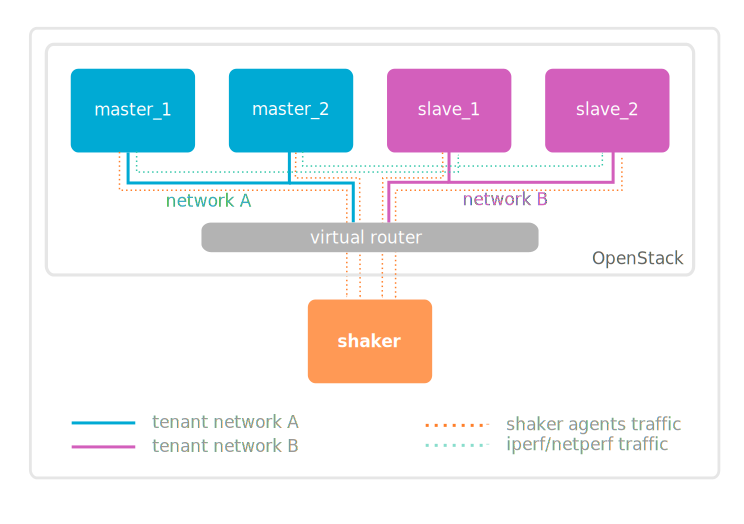
\includegraphics{architecture.jpg}
\caption{Scrapple architecture}\end{figure}
\begin{itemize}
\item {} \begin{description}
\item[{{\hyperref[framework/commands:framework-commands]{\emph{Command line input}}}}] \leavevmode
The command line input is the basis of definition of the implementation of the extractor. It specifies the project configuration and the options related to implementing the extractor.

\end{description}

\item {} \begin{description}
\item[{{\hyperref[framework/config:framework-config]{\emph{Configuration file}}}}] \leavevmode
The configuration file specifies the rules of the required extractor. It contains the selector expressions for the data to be extracted and the specification of the link crawler.

\end{description}

\item {} \begin{description}
\item[{{\hyperref[concepts/selectors:concepts-selectors]{\emph{Extractor framework}}}}] \leavevmode
The extractor framework handles the implementation of the parsing \& extraction. The extractor framework follows the following steps :
\begin{itemize}
\item {} 
It makes HTTP requests to fetch the web page to be parsed.

\item {} 
It parses through the {\hyperref[concepts/structure:concepts-structure]{\emph{element tree}}}.

\item {} 
It extracts the required content, depending on the extractor rules in the configuration file.

\item {} 
In case of crawlers, this process is repeated for all the pages that the extractor crawls through.

\end{itemize}

\end{description}

\item {} \begin{description}
\item[{{\hyperref[concepts/formats:concepts-formats]{\emph{Data format handler}}}}] \leavevmode
According to the options specified in the CLI input, the extracted content is stored as a CSV document or a JSON document.

\end{description}

\end{itemize}


\section{Scrapple commands}
\label{framework/commands:scrapple-commands}\label{framework/commands::doc}\label{framework/commands:framework-commands}
The four commands provided by the Scrapple CLI are
\begin{itemize}
\item {} 
genconfig

\item {} 
generate

\item {} 
run

\item {} 
web

\end{itemize}


\subsection{genconfig}
\label{framework/commands:command-genconfig}\label{framework/commands:genconfig}
The \code{genconfig} command is used to create a skeleton {\hyperref[framework/config:framework-config]{\emph{configuration file}}}, which can be used as the base for further writing the necessary configuration file. This makes it easier to understand the structure of the key/value-based configuration file, and provide the necessary options.

The two positional arguments for the genconfig command are :
\begin{itemize}
\item {} 
The project name

\item {} 
The base URL

\end{itemize}

The \code{genconfig} command creates a basic configuration file with the provided base URL, and creates it as ``\textless{}project\_name\textgreater{}.json''.

The two optional arguments for the genconfig command are :
\begin{itemize}
\item {} 
The type of extractor

\item {} 
The selector type

\end{itemize}

The extractor could be a scraper or a crawler, and this can be specified in the --type argument. By default, it is a scraper. When the crawler option is provided, it adds the ``next'' parameter in the skeleton configuration file.

With the --selector option, the selector type to be used can be specified. This can be ``css'' or ``xpath''. By default, it is ``xpath''.

Examples :
\begin{itemize}
\item {} 
\code{\$ scrapple genconfig pyvideo http://pyvideo.org/category} creates pyvideo.json, which contains the skeleton configuration file for a scraper which uses XPath expressions as the selector.

\item {} 
\code{\$ scrapple genconfig pyvideo http://pyvideo.org/category -{-}type=crawler} creates pyvideo.json, which contains the skeleton configuration file for a crawler which uses XPath expressions as the selector.

\item {} 
\code{\$ scrapple genconfig pyvideo http://pyvideo.org/category -{-}type=crawler -{-}selector=css} creates pyvideo.json, which contains the skeleton configuration file for a crawler which uses CSS selector expressions as the selector.

\end{itemize}


\subsection{generate}
\label{framework/commands:command-generate}\label{framework/commands:generate}
The \code{generate} command is used to generate the Python script corresponding to the specifications in the configuration file. This command is used to create the script that replicates the operation of the run command.

The two positional arguments for the generate command are :
\begin{itemize}
\item {} 
The project name

\item {} 
The output file name

\end{itemize}

The project name is the name of the configuration file to be used, i.e, ``\textless{}project\_name\textgreater{}.json'' is the configuration file used as the specification. The command creates ``\textless{}output\_file\_name\textgreater{}.py'' as the generated Python script.

The one available optional argument is :
\begin{itemize}
\item {} 
The output type

\end{itemize}

This specifies the output format in which the extracted content is to be stored. This could be ``csv'' or ``json''. By default, it is ``json''.

Examples :
\begin{itemize}
\item {} 
\code{\$ scrapple generate pyvideo talk1} generates talk1.py based on pyvideo.json, where the extracted data is stored in a JSON document.

\item {} 
\code{\$ scrapple generate pyvideo talk1 -{-}output\_type=csv} generates talk1.py based on pyvideo.json, where the extracted data is stored in a CSV document.

\end{itemize}


\subsection{run}
\label{framework/commands:command-run}\label{framework/commands:run}
The \code{run} command is used to run the extractor corresponding to the specifications in the configuration file. This command runs the extractors and stores the extracted content for later use.

The two positional arguments for the generate command are :
\begin{itemize}
\item {} 
The project name

\item {} 
The output file name

\end{itemize}

The project name is the name of the configuration file to be used, i.e, ``\textless{}project\_name\textgreater{}.json'' is the configuration file used as the specification. The command creates ``\textless{}output\_file\_name\textgreater{}.json'' or ``\textless{}output\_file\_name\textgreater{}.csv'' which contains the extracted content.

The one available optional argument is :
\begin{itemize}
\item {} 
The output type

\end{itemize}

This specifies the output format in which the extracted content is to be stored. This could be ``csv'' or ``json''. By default, it is ``json''.

Examples :
\begin{itemize}
\item {} 
\code{\$ scrapple run pyvideo talk1} runs the extractor based on pyvideo.json, and stores the extracted content in talk1.json.

\item {} 
\code{\$ scrapple run pyvideo talk1 -{-}output\_type=csv} runs the extractor based on pyvideo.json, and stores the extracted content in talk1.csv.

\end{itemize}


\subsection{web}
\label{framework/commands:web}\label{framework/commands:command-web}
The \code{web} command is an added feature, to make it easier to edit the configuration file. It provides a web interface, which contains a form where the configuration file can be filled. It currently supports only editing configuration files for scrapers. Future work includes support for editing configuration files for link crawlers.

The web interface can be opened with the command

\code{\$ scrapple web}

This starts a Flask web app, which opens on port 5000 on the localhost.


\section{Configuration file}
\label{framework/config:configuration-file}\label{framework/config::doc}\label{framework/config:framework-config}
The configuration file is the basic specification of the extractor required. It contains the URL for the web page to be loaded, the selector expressions for the data to be extracted and in the case of crawlers, the selector expression for the links to be crawled through.

The keys used in the configuration file are :
\begin{itemize}
\item {} 
\textbf{project\_name} : Specifies the name of the project with which the configuration file is associated.

\item {} 
\textbf{selector\_type} : Specifies the type of selector expressions used. This could be ``xpath'' or ``css''.

\item {} \begin{description}
\item[{\textbf{scraping}}] \leavevmode{[}Specifies parameters for the extractor to be created.{]}\begin{itemize}
\item {} 
\textbf{url} : Specifies the URL of the base web page to be loaded.

\item {} \begin{description}
\item[{\textbf{data}}] \leavevmode{[}Specifies a list of selectors for the data to be extracted.{]}\begin{itemize}
\item {} 
\textbf{selector} : Specifies the selector expression.

\item {} 
\textbf{attr} : Specifies the attribute to be extracted from the result of the selector expression.

\item {} 
\textbf{field} : Specifies the field name under which this data is to stored.

\item {} 
\textbf{default} : Specifies the default value to be used if the selector expression fails.

\end{itemize}

\end{description}

\item {} \begin{description}
\item[{\textbf{next}}] \leavevmode{[}Specifies the crawler implementation.{]}\begin{itemize}
\item {} 
\textbf{follow\_link} : Specifies the selector expression for the \code{\textless{}a\textgreater{}} tags to be crawled through.

\end{itemize}

\end{description}

\end{itemize}

\end{description}

\end{itemize}

The main objective of the configuration file is to specify extraction rules in terms of selector expressions and the attribute to be extracted. There are certain set forms of selector/attribute value pairs that perform various types of content extraction.

Selector expressions :
\begin{itemize}
\item {} 
CSS selector or XPath expressions that specify the tag to be selected.

\item {} 
``url'' to take the URL of the current page on which extraction is being performed.

\end{itemize}

Attribute selectors :
\begin{itemize}
\item {} 
``text'' to extract the textual content from that tag.

\item {} 
``href'', ``src'' etc., to extract any of the other attributes of the selected tag.

\end{itemize}


\section{Scrapple implementation classes}
\label{implementation/classes:implementation-classes}\label{implementation/classes::doc}\label{implementation/classes:scrapple-implementation-classes}
There are two main categories of classes involved in the implementation of extractors on Scrapple :
\begin{itemize}
\item {} 
{\hyperref[implementation/commands:implementation-commands]{\emph{Command classes}}}

\item {} 
{\hyperref[implementation/selectors:implementation-selectors]{\emph{Selector classes}}}

\end{itemize}

\textbf{Command classes} define the execution of the commands provided by Scrapple.

\textbf{Selector classes} define the implementation of the extraction through the selector expressions.

The following class diagram can be used to represent the relationship between the various classes.
\begin{figure}[htbp]
\centering
\capstart

\includegraphics{class.png}
\caption{Scrapple class diagram}\end{figure}


\section{Command line interface}
\label{implementation/cli:implementation-cli}\label{implementation/cli:command-line-interface}\label{implementation/cli::doc}
Scrapple is primarily run through a command line interface. The CLI is used to execute the {\hyperref[framework/commands:framework-commands]{\emph{commands supported by Scrapple}}}. For a description of the usage of the Scrapple CLI, the help option can be used.

\code{\$ scrapple -{-}help}

This presents the usage description and an explanation of the optional arguments provided by the commands.

\begin{Verbatim}[commandchars=\\\{\}]
Usage:
    scrapple (\PYGZhy{}h \textbar{} \PYGZhy{}\PYGZhy{}help \textbar{} \PYGZhy{}\PYGZhy{}version)
    scrapple genconfig \PYGZlt{}projectname\PYGZgt{} \PYGZlt{}url\PYGZgt{} [\PYGZhy{}\PYGZhy{}type=\PYGZlt{}type\PYGZgt{}] [\PYGZhy{}\PYGZhy{}selector=\PYGZlt{}selector\PYGZgt{}]
    scrapple run \PYGZlt{}projectname\PYGZgt{} \PYGZlt{}output\PYGZus{}filename\PYGZgt{} [\PYGZhy{}\PYGZhy{}output\PYGZus{}type=\PYGZlt{}output\PYGZus{}type\PYGZgt{}]
    scrapple generate \PYGZlt{}projectname\PYGZgt{} \PYGZlt{}output\PYGZus{}filename\PYGZgt{} [\PYGZhy{}\PYGZhy{}output\PYGZus{}type=\PYGZlt{}output\PYGZus{}type\PYGZgt{}]
    scrapple web

Options:
    \PYGZhy{}h, \PYGZhy{}\PYGZhy{}help
        Show this help message and exit
    \PYGZhy{}\PYGZhy{}version
        Display the version of Scrapple
    \PYGZhy{}\PYGZhy{}type=\PYGZlt{}type\PYGZgt{}, \PYGZhy{}t \PYGZlt{}type\PYGZgt{}
        Specifies if the script generated is a page scraper or a crawler [default: scraper]
    \PYGZhy{}\PYGZhy{}selector=\PYGZlt{}selector\PYGZgt{}, \PYGZhy{}s \PYGZlt{}selector\PYGZgt{}
        Specifies if XPath expressions or CSS selectors are used [default: xpath]
    \PYGZhy{}\PYGZhy{}output\PYGZus{}type=\PYGZlt{}output\PYGZus{}type\PYGZgt{}, \PYGZhy{}o \PYGZlt{}output\PYGZus{}type\PYGZgt{}
        Specifies if the generated output is stored as CSV or JSON [default: json]
\end{Verbatim}

The \code{scrapple} tool on the command line is included in the system path when Scrapple is {\hyperref[intro/install:intro-install]{\emph{installed}}}. When the tool is run, the input on the CLI is parsed by the runCLI() function.
\index{runCLI() (in module scrapple.cmd)}

\begin{fulllineitems}
\phantomsection\label{implementation/cli:scrapple.cmd.runCLI}\pysiglinewithargsret{\code{scrapple.cmd.}\bfcode{runCLI}}{}{}
The starting point for the execution of the Scrapple command line tool.

runCLI uses the docstring as the usage description for the scrapple command.     The class for the required command is selected by a dynamic dispatch, and the     command is executed through the execute\_command() method of the command class.

\end{fulllineitems}


This functionality is implemented by the following code block -

\begin{Verbatim}[commandchars=\\\{\}]
\PYG{n}{handle\PYGZus{}exceptions}\PYG{p}{(}\PYG{n}{args}\PYG{p}{)}
\PYG{n}{command\PYGZus{}list} \PYG{o}{=} \PYG{p}{[}\PYG{l+s}{\PYGZsq{}}\PYG{l+s}{genconfig}\PYG{l+s}{\PYGZsq{}}\PYG{p}{,} \PYG{l+s}{\PYGZsq{}}\PYG{l+s}{run}\PYG{l+s}{\PYGZsq{}}\PYG{p}{,} \PYG{l+s}{\PYGZsq{}}\PYG{l+s}{generate}\PYG{l+s}{\PYGZsq{}}\PYG{p}{,} \PYG{l+s}{\PYGZsq{}}\PYG{l+s}{web}\PYG{l+s}{\PYGZsq{}}\PYG{p}{]}
\PYG{n}{select} \PYG{o}{=} \PYG{n}{itemgetter}\PYG{p}{(}\PYG{l+s}{\PYGZsq{}}\PYG{l+s}{genconfig}\PYG{l+s}{\PYGZsq{}}\PYG{p}{,} \PYG{l+s}{\PYGZsq{}}\PYG{l+s}{run}\PYG{l+s}{\PYGZsq{}}\PYG{p}{,} \PYG{l+s}{\PYGZsq{}}\PYG{l+s}{generate}\PYG{l+s}{\PYGZsq{}}\PYG{p}{,} \PYG{l+s}{\PYGZsq{}}\PYG{l+s}{web}\PYG{l+s}{\PYGZsq{}}\PYG{p}{)}
\PYG{n}{selectedCommand} \PYG{o}{=} \PYG{n}{command\PYGZus{}list}\PYG{p}{[}\PYG{n}{select}\PYG{p}{(}\PYG{n}{args}\PYG{p}{)}\PYG{o}{.}\PYG{n}{index}\PYG{p}{(}\PYG{n+nb+bp}{True}\PYG{p}{)}\PYG{p}{]}
\PYG{n}{cmdClass} \PYG{o}{=} \PYG{n}{get\PYGZus{}command\PYGZus{}class}\PYG{p}{(}\PYG{n}{selectedCommand}\PYG{p}{)}
\PYG{n}{obj} \PYG{o}{=} \PYG{n}{cmdClass}\PYG{p}{(}\PYG{n}{args}\PYG{p}{)}
\PYG{n}{obj}\PYG{o}{.}\PYG{n}{execute\PYGZus{}command}\PYG{p}{(}\PYG{p}{)}
\end{Verbatim}


\section{Command classes}
\label{implementation/commands:command-classes}\label{implementation/commands::doc}\label{implementation/commands:implementation-commands}\label{implementation/commands:module-scrapple.commands.genconfig}\index{scrapple.commands.genconfig (module)}

\subsection{scrapple.commands.genconfig}
\label{implementation/commands:scrapple-commands-genconfig}\index{GenconfigCommand (class in scrapple.commands.genconfig)}

\begin{fulllineitems}
\phantomsection\label{implementation/commands:scrapple.commands.genconfig.GenconfigCommand}\pysiglinewithargsret{\strong{class }\code{scrapple.commands.genconfig.}\bfcode{GenconfigCommand}}{\emph{args}}{}
Defines the execution of {\hyperref[framework/commands:command-genconfig]{\emph{genconfig}}}
\index{execute\_command() (scrapple.commands.genconfig.GenconfigCommand method)}

\begin{fulllineitems}
\phantomsection\label{implementation/commands:scrapple.commands.genconfig.GenconfigCommand.execute_command}\pysiglinewithargsret{\bfcode{execute\_command}}{}{}
The genconfig command depends on predefined \href{http://jinja.pocoo.org/}{Jinja2}         templates for the skeleton configuration files. Taking the --type argument from the         CLI input, the corresponding template file is used.

Settings for the configuration file, like project name, selector type and URL         are taken from the CLI input and using these as parameters, the template is         rendered. This rendered JSON document is saved as \textless{}project\_name\textgreater{}.json.

\end{fulllineitems}


\end{fulllineitems}

\phantomsection\label{implementation/commands:module-scrapple.commands.generate}\index{scrapple.commands.generate (module)}

\subsection{scrapple.commands.generate}
\label{implementation/commands:scrapple-commands-generate}\index{GenerateCommand (class in scrapple.commands.generate)}

\begin{fulllineitems}
\phantomsection\label{implementation/commands:scrapple.commands.generate.GenerateCommand}\pysiglinewithargsret{\strong{class }\code{scrapple.commands.generate.}\bfcode{GenerateCommand}}{\emph{args}}{}
Defines the execution of {\hyperref[framework/commands:command-generate]{\emph{generate}}}
\index{execute\_command() (scrapple.commands.generate.GenerateCommand method)}

\begin{fulllineitems}
\phantomsection\label{implementation/commands:scrapple.commands.generate.GenerateCommand.execute_command}\pysiglinewithargsret{\bfcode{execute\_command}}{}{}
The generate command uses \href{http://jinja.pocoo.org/}{Jinja2} templates         to create Python scripts, according to the specification in the configuration         file. The predefined templates use the extract\_content() method of the         {\hyperref[implementation/selectors:implementation-selectors]{\emph{selector classes}}} to implement linear extractors         and use recursive for loops to implement multiple levels of link crawlers. This         implementation is effectively a representation of the traverse\_next()         {\hyperref[implementation/utils:implementation-utils]{\emph{utility function}}}, using the loop depth to         differentiate between levels of the crawler execution.

According to the --output\_type argument in the CLI input, the results are         written into a JSON document or a CSV document.

The Python script is written into \textless{}output\_filename\textgreater{}.py - running this file         is the equivalent of using the Scrapple {\hyperref[framework/commands:command-run]{\emph{run command}}}.

\end{fulllineitems}


\end{fulllineitems}

\phantomsection\label{implementation/commands:module-scrapple.commands.run}\index{scrapple.commands.run (module)}

\subsection{scrapple.commands.run}
\label{implementation/commands:scrapple-commands-run}\index{RunCommand (class in scrapple.commands.run)}

\begin{fulllineitems}
\phantomsection\label{implementation/commands:scrapple.commands.run.RunCommand}\pysiglinewithargsret{\strong{class }\code{scrapple.commands.run.}\bfcode{RunCommand}}{\emph{args}}{}
Defines the execution of {\hyperref[framework/commands:command-run]{\emph{run}}}
\index{execute\_command() (scrapple.commands.run.RunCommand method)}

\begin{fulllineitems}
\phantomsection\label{implementation/commands:scrapple.commands.run.RunCommand.execute_command}\pysiglinewithargsret{\bfcode{execute\_command}}{}{}
The run command implements the web content extractor corresponding to the given         configuration file.

The execute\_command() validates the input project name and opens the JSON         configuration file. The run() method handles the execution of the extractor run.

The extractor implementation follows these primary steps :
\begin{enumerate}
\item {} 
Selects the appropriate {\hyperref[implementation/selectors:implementation-selectors]{\emph{selector class}}} through         a dynamic dispatch, with the selector\_type argument from the CLI input.

\item {} 
Iterate through the data section in level-0 of the configuration file.         On each data item, call the extract\_content() method from the selector class to         extract the content according to the specified extractor rule.

\item {} 
If there are multiple levels of the extractor, i.e, if there is a `next'         attribute in the configuration file, call the traverse\_next()         {\hyperref[implementation/utils:implementation-utils]{\emph{utility function}}} and parse through successive levels         of the configuration file.

\item {} 
According to the --output\_type argument, the result data is saved in a JSON         document or a CSV document.

\end{enumerate}

\end{fulllineitems}


\end{fulllineitems}

\phantomsection\label{implementation/commands:module-scrapple.commands.web}\index{scrapple.commands.web (module)}

\subsection{scrapple.commands.web}
\label{implementation/commands:scrapple-commands-web}\index{WebCommand (class in scrapple.commands.web)}

\begin{fulllineitems}
\phantomsection\label{implementation/commands:scrapple.commands.web.WebCommand}\pysiglinewithargsret{\strong{class }\code{scrapple.commands.web.}\bfcode{WebCommand}}{\emph{args}}{}
Defines the execution of {\hyperref[framework/commands:command-web]{\emph{web}}}
\index{execute\_command() (scrapple.commands.web.WebCommand method)}

\begin{fulllineitems}
\phantomsection\label{implementation/commands:scrapple.commands.web.WebCommand.execute_command}\pysiglinewithargsret{\bfcode{execute\_command}}{}{}
The web command runs the Scrapple web interface through a simple         \href{http://flask.pocoo.org}{Flask} app.

When the execute\_command() method is called from the         {\hyperref[implementation/cli:implementation-cli]{\emph{runCLI()}}} function, it starts of two simultaneous         processes :
\begin{itemize}
\item {} 
Calls the run\_flask() method to start the Flask app on port 5000 of localhost

\item {} 
Opens the web interface on a web browser

\end{itemize}

The `/' view of the Flask app, opens up the Scrapple web interface. This         provides a basic form, to fill in the required configuration file. On submitting         the form, it makes a POST request, passing in the form in the request header.         This form is passed to the form\_to\_json()         {\hyperref[implementation/utils:implementation-utils]{\emph{utility function}}}, where the form is converted into         the resultant JSON configuration file.

Currently, closing the web command execution requires making a keyboard interrupt         on the command line after the web interface has been closed.

\end{fulllineitems}


\end{fulllineitems}



\section{Selector classes}
\label{implementation/selectors:selector-classes}\label{implementation/selectors::doc}\label{implementation/selectors:implementation-selectors}
{\hyperref[concepts/selectors:concepts-selectors]{\emph{Selectors}}} are used to specifically point to certain tags on a web page, from which content has to be extracted. In Scrapple, selectors are implemented through selector classes, which define methods to extract necessary content through specified selector expressions and to extract links from anchor tags to be crawled through.

There are two selector types that are supported in Scrapple :
\begin{itemize}
\item {} 
XPath expressions

\item {} 
CSS selector expressions

\end{itemize}

These selector types are implemented through the \code{XpathSelector} and \code{CssSelector} classes, respectively. These two classes use the \code{Selector} class as their super class.

In the super class, the URL of the web page to be loaded is validated - ensuring the schema has been specified, and that the URL is valid. A HTTP GET request is made to load the web page, and the HTML content of this fetched web page is used to generate the {\hyperref[concepts/structure:concepts-structure]{\emph{element tree}}}. This is the element tree that will be parsed to extract the necessary content.
\phantomsection\label{implementation/selectors:module-scrapple.selectors.xpath}\index{scrapple.selectors.xpath (module)}

\subsection{scrapple.selectors.xpath}
\label{implementation/selectors:scrapple-selectors-xpath}\index{XpathSelector (class in scrapple.selectors.xpath)}

\begin{fulllineitems}
\phantomsection\label{implementation/selectors:scrapple.selectors.xpath.XpathSelector}\pysiglinewithargsret{\strong{class }\code{scrapple.selectors.xpath.}\bfcode{XpathSelector}}{\emph{url}}{}
The \code{XpathSelector} object defines XPath expressions.
\index{extract\_content() (scrapple.selectors.xpath.XpathSelector method)}

\begin{fulllineitems}
\phantomsection\label{implementation/selectors:scrapple.selectors.xpath.XpathSelector.extract_content}\pysiglinewithargsret{\bfcode{extract\_content}}{\emph{selector}, \emph{attr}, \emph{default}}{}
Method for performing the content extraction for the given XPath expression.

The XPath selector expression can be used to extract content            from the element tree corresponding to the fetched web page.

If the selector is ``url'', the URL of the current web page is returned.
Otherwise, the selector expression is used to extract content. The particular           attribute to be extracted (``text'', ``href'', etc.) is specified in the method             arguments, and this is used to extract the required content. If the content             extracted is a link (from an attr value of ``href'' or ``src''), the URL is parsed          to convert the relative path into an absolute path.

If the selector does not fetch any content, the default value is returned.              If no default value is specified, an exception is raised.
\begin{quote}\begin{description}
\item[{Parameters}] \leavevmode\begin{itemize}
\item {} 
\textbf{selector} -- The XPath expression

\item {} 
\textbf{attr} -- The attribute to be extracted from the selected tag

\item {} 
\textbf{default} -- The default value to be used if the selector does not return any data

\end{itemize}

\item[{Returns}] \leavevmode
The extracted content

\end{description}\end{quote}

\end{fulllineitems}

\index{extract\_links() (scrapple.selectors.xpath.XpathSelector method)}

\begin{fulllineitems}
\phantomsection\label{implementation/selectors:scrapple.selectors.xpath.XpathSelector.extract_links}\pysiglinewithargsret{\bfcode{extract\_links}}{\emph{selector}}{}
Method for performing the link extraction for the crawler.

The selector passed as the argument is a selector to point to the anchor tags           that the crawler should pass through. A list of links is obtained, and the links                are iterated through. The relative paths are converted into absolute paths and          a \code{CssSelector} object is created with the URL of the next page as the argument               and this created object is yielded.

The extract\_links method basically generates \code{CssSelector} objects for all of                 the links to be crawled through.
\begin{quote}\begin{description}
\item[{Parameters}] \leavevmode
\textbf{selector} -- The selector for the anchor tags to be crawled through

\item[{Returns}] \leavevmode
A \code{CssSelector} object for every page to be crawled through

\end{description}\end{quote}

\end{fulllineitems}


\end{fulllineitems}

\phantomsection\label{implementation/selectors:module-scrapple.selectors.css}\index{scrapple.selectors.css (module)}

\subsection{scrapple.selectors.css}
\label{implementation/selectors:scrapple-selectors-css}\index{CssSelector (class in scrapple.selectors.css)}

\begin{fulllineitems}
\phantomsection\label{implementation/selectors:scrapple.selectors.css.CssSelector}\pysiglinewithargsret{\strong{class }\code{scrapple.selectors.css.}\bfcode{CssSelector}}{\emph{url}}{}
The \code{CssSelector} object defines CSS selector expressions.
\index{extract\_content() (scrapple.selectors.css.CssSelector method)}

\begin{fulllineitems}
\phantomsection\label{implementation/selectors:scrapple.selectors.css.CssSelector.extract_content}\pysiglinewithargsret{\bfcode{extract\_content}}{\emph{selector}, \emph{attr}, \emph{default}}{}
Method for performing the content extraction for the given CSS selector.

The cssselect library is used to handle CSS selector expressions.               XPath expressions have a higher speed of execution, so the given CSS selector           expression is translated into the corresponding XPath expression, by the                \code{cssselect.CSSSelector} class. This selector can be used to extract content           from the element tree corresponding to the fetched web page.

If the selector is ``url'', the URL of the current web page is returned.
Otherwise, the selector expression is used to extract content. The particular           attribute to be extracted (``text'', ``href'', etc.) is specified in the method             arguments, and this is used to extract the required content. If the content             extracted is a link (from an attr value of ``href'' or ``src''), the URL is parsed          to convert the relative path into an absolute path.

If the selector does not fetch any content, the default value is returned.              If no default value is specified, an exception is raised.
\begin{quote}\begin{description}
\item[{Parameters}] \leavevmode\begin{itemize}
\item {} 
\textbf{selector} -- The CSS selector expression

\item {} 
\textbf{attr} -- The attribute to be extracted from the selected tag

\item {} 
\textbf{default} -- The default value to be used if the selector does not return any data

\end{itemize}

\item[{Returns}] \leavevmode
The extracted content

\end{description}\end{quote}

\end{fulllineitems}

\index{extract\_links() (scrapple.selectors.css.CssSelector method)}

\begin{fulllineitems}
\phantomsection\label{implementation/selectors:scrapple.selectors.css.CssSelector.extract_links}\pysiglinewithargsret{\bfcode{extract\_links}}{\emph{selector}}{}
Method for performing the link extraction for the crawler implementation.

As in the extract\_content method, the cssselect library is used to translate            the CSS selector expression into an XPath expression.

The selector passed as the argument is a selector to point to the anchor tags           that the crawler should pass through. A list of links is obtained, and the links                are iterated through. The relative paths are converted into absolute paths and          a \code{CssSelector} object is created with the URL of the next page as the argument               and this created object is yielded.

The extract\_links method basically generates \code{CssSelector} objects for all of                 the links to be crawled through.
\begin{quote}\begin{description}
\item[{Parameters}] \leavevmode
\textbf{selector} -- The selector for the anchor tags to be crawled through

\item[{Returns}] \leavevmode
A \code{CssSelector} object for every page to be crawled through

\end{description}\end{quote}

\end{fulllineitems}


\end{fulllineitems}



\section{Utility functions}
\label{implementation/utils::doc}\label{implementation/utils:module-scrapple.utils.dynamicdispatch}\label{implementation/utils:implementation-utils}\label{implementation/utils:utility-functions}\index{scrapple.utils.dynamicdispatch (module)}

\subsection{scrapple.utils.dynamicdispatch}
\label{implementation/utils:scrapple-utils-dynamicdispatch}
Functions related to dynamic dispatch of objects
\index{get\_command\_class() (in module scrapple.utils.dynamicdispatch)}

\begin{fulllineitems}
\phantomsection\label{implementation/utils:scrapple.utils.dynamicdispatch.get_command_class}\pysiglinewithargsret{\code{scrapple.utils.dynamicdispatch.}\bfcode{get\_command\_class}}{\emph{command}}{}
Called from runCLI() to select the command class for the selected command.
\begin{quote}\begin{description}
\item[{Parameters}] \leavevmode
\textbf{command} -- The command to be implemented

\item[{Returns}] \leavevmode
The command class corresponding to the selected command

\end{description}\end{quote}

\end{fulllineitems}


This function is implemented through this simple code block :

\begin{Verbatim}[commandchars=\\\{\}]
\PYG{k+kn}{from} \PYG{n+nn}{scrapple.commands} \PYG{k+kn}{import} \PYG{n}{genconfig}\PYG{p}{,} \PYG{n}{generate}\PYG{p}{,} \PYG{n}{run}\PYG{p}{,} \PYG{n}{web}
\PYG{n}{cmdClass} \PYG{o}{=} \PYG{n+nb}{getattr}\PYG{p}{(}\PYG{n+nb}{eval}\PYG{p}{(}\PYG{n}{command}\PYG{p}{)}\PYG{p}{,} \PYG{n}{command}\PYG{o}{.}\PYG{n}{title}\PYG{p}{(}\PYG{p}{)} \PYG{o}{+} \PYG{l+s}{\PYGZsq{}}\PYG{l+s}{Command}\PYG{l+s}{\PYGZsq{}}\PYG{p}{)}
\PYG{k}{return} \PYG{n}{cmdClass}
\end{Verbatim}
\phantomsection\label{implementation/utils:module-scrapple.utils.exceptions}\index{scrapple.utils.exceptions (module)}

\subsection{scrapple.utils.exceptions}
\label{implementation/utils:scrapple-utils-exceptions}
Functions related to handling exceptions in the input arguments
\index{handle\_exceptions() (in module scrapple.utils.exceptions)}

\begin{fulllineitems}
\phantomsection\label{implementation/utils:scrapple.utils.exceptions.handle_exceptions}\pysiglinewithargsret{\code{scrapple.utils.exceptions.}\bfcode{handle\_exceptions}}{\emph{args}}{}
Validates the arguments passed through the CLI commands.
\begin{quote}\begin{description}
\item[{Parameters}] \leavevmode
\textbf{args} -- The arguments passed in the CLI, parsed by the docopt module

\item[{Returns}] \leavevmode
None

\end{description}\end{quote}

\end{fulllineitems}


The function uses regular expressions to validate the CLI input.

\begin{Verbatim}[commandchars=\\\{\}]
\PYG{n}{projectname\PYGZus{}re} \PYG{o}{=} \PYG{n}{re}\PYG{o}{.}\PYG{n}{compile}\PYG{p}{(}\PYG{l+s}{r\PYGZsq{}}\PYG{l+s}{[\PYGZca{}a\PYGZhy{}zA\PYGZhy{}Z0\PYGZhy{}9\PYGZus{}]}\PYG{l+s}{\PYGZsq{}}\PYG{p}{)}
\PYG{k}{if} \PYG{n}{args}\PYG{p}{[}\PYG{l+s}{\PYGZsq{}}\PYG{l+s}{genconfig}\PYG{l+s}{\PYGZsq{}}\PYG{p}{]}\PYG{p}{:}
        \PYG{k}{if} \PYG{n}{args}\PYG{p}{[}\PYG{l+s}{\PYGZsq{}}\PYG{l+s}{\PYGZhy{}\PYGZhy{}type}\PYG{l+s}{\PYGZsq{}}\PYG{p}{]} \PYG{o+ow}{not} \PYG{o+ow}{in} \PYG{p}{[}\PYG{l+s}{\PYGZsq{}}\PYG{l+s}{scraper}\PYG{l+s}{\PYGZsq{}}\PYG{p}{,} \PYG{l+s}{\PYGZsq{}}\PYG{l+s}{crawler}\PYG{l+s}{\PYGZsq{}}\PYG{p}{]}\PYG{p}{:}
                \PYG{k}{raise} \PYG{n+ne}{Exception}\PYG{p}{(}\PYG{l+s}{\PYGZdq{}}\PYG{l+s}{\PYGZhy{}\PYGZhy{}type has to be }\PYG{l+s}{\PYGZsq{}}\PYG{l+s}{scraper}\PYG{l+s}{\PYGZsq{}}\PYG{l+s}{ or }\PYG{l+s}{\PYGZsq{}}\PYG{l+s}{crawler}\PYG{l+s}{\PYGZsq{}}\PYG{l+s}{\PYGZdq{}}\PYG{p}{)}
        \PYG{k}{if} \PYG{n}{args}\PYG{p}{[}\PYG{l+s}{\PYGZsq{}}\PYG{l+s}{\PYGZhy{}\PYGZhy{}selector}\PYG{l+s}{\PYGZsq{}}\PYG{p}{]} \PYG{o+ow}{not} \PYG{o+ow}{in} \PYG{p}{[}\PYG{l+s}{\PYGZsq{}}\PYG{l+s}{xpath}\PYG{l+s}{\PYGZsq{}}\PYG{p}{,} \PYG{l+s}{\PYGZsq{}}\PYG{l+s}{css}\PYG{l+s}{\PYGZsq{}}\PYG{p}{]}\PYG{p}{:}
                \PYG{k}{raise} \PYG{n+ne}{Exception}\PYG{p}{(}\PYG{l+s}{\PYGZdq{}}\PYG{l+s}{\PYGZhy{}\PYGZhy{}selector has to be }\PYG{l+s}{\PYGZsq{}}\PYG{l+s}{xpath}\PYG{l+s}{\PYGZsq{}}\PYG{l+s}{ or }\PYG{l+s}{\PYGZsq{}}\PYG{l+s}{css}\PYG{l+s}{\PYGZsq{}}\PYG{l+s}{\PYGZdq{}}\PYG{p}{)}
\PYG{k}{if} \PYG{n}{args}\PYG{p}{[}\PYG{l+s}{\PYGZsq{}}\PYG{l+s}{generate}\PYG{l+s}{\PYGZsq{}}\PYG{p}{]} \PYG{o+ow}{or} \PYG{n}{args}\PYG{p}{[}\PYG{l+s}{\PYGZsq{}}\PYG{l+s}{run}\PYG{l+s}{\PYGZsq{}}\PYG{p}{]}\PYG{p}{:}
        \PYG{k}{if} \PYG{n}{args}\PYG{p}{[}\PYG{l+s}{\PYGZsq{}}\PYG{l+s}{\PYGZhy{}\PYGZhy{}output\PYGZus{}type}\PYG{l+s}{\PYGZsq{}}\PYG{p}{]} \PYG{o+ow}{not} \PYG{o+ow}{in} \PYG{p}{[}\PYG{l+s}{\PYGZsq{}}\PYG{l+s}{json}\PYG{l+s}{\PYGZsq{}}\PYG{p}{,} \PYG{l+s}{\PYGZsq{}}\PYG{l+s}{csv}\PYG{l+s}{\PYGZsq{}}\PYG{p}{]}\PYG{p}{:}
                \PYG{k}{raise} \PYG{n+ne}{Exception}\PYG{p}{(}\PYG{l+s}{\PYGZdq{}}\PYG{l+s}{\PYGZhy{}\PYGZhy{}output\PYGZus{}type has to be }\PYG{l+s}{\PYGZsq{}}\PYG{l+s}{json}\PYG{l+s}{\PYGZsq{}}\PYG{l+s}{ or }\PYG{l+s}{\PYGZsq{}}\PYG{l+s}{csv}\PYG{l+s}{\PYGZsq{}}\PYG{l+s}{\PYGZdq{}}\PYG{p}{)}
\PYG{k}{if} \PYG{n}{args}\PYG{p}{[}\PYG{l+s}{\PYGZsq{}}\PYG{l+s}{genconfig}\PYG{l+s}{\PYGZsq{}}\PYG{p}{]} \PYG{o+ow}{or} \PYG{n}{args}\PYG{p}{[}\PYG{l+s}{\PYGZsq{}}\PYG{l+s}{generate}\PYG{l+s}{\PYGZsq{}}\PYG{p}{]} \PYG{o+ow}{or} \PYG{n}{args}\PYG{p}{[}\PYG{l+s}{\PYGZsq{}}\PYG{l+s}{run}\PYG{l+s}{\PYGZsq{}}\PYG{p}{]}\PYG{p}{:}
        \PYG{k}{if} \PYG{n}{projectname\PYGZus{}re}\PYG{o}{.}\PYG{n}{search}\PYG{p}{(}\PYG{n}{args}\PYG{p}{[}\PYG{l+s}{\PYGZsq{}}\PYG{l+s}{\PYGZlt{}projectname\PYGZgt{}}\PYG{l+s}{\PYGZsq{}}\PYG{p}{]}\PYG{p}{)} \PYG{o+ow}{is} \PYG{o+ow}{not} \PYG{n+nb+bp}{None}\PYG{p}{:}
                \PYG{k}{raise} \PYG{n+ne}{Exception}\PYG{p}{(}\PYG{l+s}{\PYGZdq{}}\PYG{l+s}{Invalid \PYGZlt{}projectname\PYGZgt{}}\PYG{l+s}{\PYGZdq{}}\PYG{p}{)}
\PYG{k}{return}
\end{Verbatim}
\phantomsection\label{implementation/utils:module-scrapple.utils.config}\index{scrapple.utils.config (module)}

\subsection{scrapple.utils.config}
\label{implementation/utils:scrapple-utils-config}
Functions related to traversing the configuration file
\index{traverse\_next() (in module scrapple.utils.config)}

\begin{fulllineitems}
\phantomsection\label{implementation/utils:scrapple.utils.config.traverse_next}\pysiglinewithargsret{\code{scrapple.utils.config.}\bfcode{traverse\_next}}{\emph{page}, \emph{next}, \emph{results}}{}
Recursive generator to traverse through the next attribute and     crawl through the links to be followed.
\begin{quote}\begin{description}
\item[{Parameters}] \leavevmode\begin{itemize}
\item {} 
\textbf{page} -- The current page being parsed

\item {} 
\textbf{next} -- The next attribute of the current scraping dict

\item {} 
\textbf{results} -- The current extracted content, stored in a dict

\end{itemize}

\item[{Returns}] \leavevmode
The extracted content, through a generator

\end{description}\end{quote}

\end{fulllineitems}


In the case of crawlers, the configuration file can be treated as a tree, with the anchor tag links extracted from the follow link selector as the child nodes. This level-wise representation of the crawler configuration file provides a clear picture of how the file should be parsed.
\begin{figure}[htbp]
\centering
\capstart

\includegraphics{tree.jpg}
\caption{Tree representation of crawler}\end{figure}

This recursive generator performs a depth-first traversal of the config file tree. It can be implemented through this code snippet :

\begin{Verbatim}[commandchars=\\\{\}]
\PYG{k}{for} \PYG{n}{link} \PYG{o+ow}{in} \PYG{n}{page}\PYG{o}{.}\PYG{n}{extract\PYGZus{}links}\PYG{p}{(}\PYG{n+nb}{next}\PYG{p}{[}\PYG{l+s}{\PYGZsq{}}\PYG{l+s}{follow\PYGZus{}link}\PYG{l+s}{\PYGZsq{}}\PYG{p}{]}\PYG{p}{)}\PYG{p}{:}
        \PYG{n}{r} \PYG{o}{=} \PYG{n}{results}\PYG{o}{.}\PYG{n}{copy}\PYG{p}{(}\PYG{p}{)}
        \PYG{k}{for} \PYG{n}{attribute} \PYG{o+ow}{in} \PYG{n+nb}{next}\PYG{p}{[}\PYG{l+s}{\PYGZsq{}}\PYG{l+s}{scraping}\PYG{l+s}{\PYGZsq{}}\PYG{p}{]}\PYG{o}{.}\PYG{n}{get}\PYG{p}{(}\PYG{l+s}{\PYGZsq{}}\PYG{l+s}{data}\PYG{l+s}{\PYGZsq{}}\PYG{p}{)}\PYG{p}{:}
                \PYG{k}{if} \PYG{n}{attribute}\PYG{p}{[}\PYG{l+s}{\PYGZsq{}}\PYG{l+s}{field}\PYG{l+s}{\PYGZsq{}}\PYG{p}{]} \PYG{o}{!=} \PYG{l+s}{\PYGZdq{}}\PYG{l+s}{\PYGZdq{}}\PYG{p}{:}
                        \PYG{n}{r}\PYG{p}{[}\PYG{n}{attribute}\PYG{p}{[}\PYG{l+s}{\PYGZsq{}}\PYG{l+s}{field}\PYG{l+s}{\PYGZsq{}}\PYG{p}{]}\PYG{p}{]} \PYG{o}{=} \PYGZbs{}
                        \PYG{n}{link}\PYG{o}{.}\PYG{n}{extract\PYGZus{}content}\PYG{p}{(}\PYG{n}{attribute}\PYG{p}{[}\PYG{l+s}{\PYGZsq{}}\PYG{l+s}{selector}\PYG{l+s}{\PYGZsq{}}\PYG{p}{]}\PYG{p}{,}
                        \PYG{n}{attribute}\PYG{p}{[}\PYG{l+s}{\PYGZsq{}}\PYG{l+s}{attr}\PYG{l+s}{\PYGZsq{}}\PYG{p}{]}\PYG{p}{,}
                        \PYG{n}{attribute}\PYG{p}{[}\PYG{l+s}{\PYGZsq{}}\PYG{l+s}{default}\PYG{l+s}{\PYGZsq{}}\PYG{p}{]}\PYG{p}{)}
        \PYG{k}{if} \PYG{o+ow}{not} \PYG{n+nb}{next}\PYG{p}{[}\PYG{l+s}{\PYGZsq{}}\PYG{l+s}{scraping}\PYG{l+s}{\PYGZsq{}}\PYG{p}{]}\PYG{o}{.}\PYG{n}{get}\PYG{p}{(}\PYG{l+s}{\PYGZsq{}}\PYG{l+s}{next}\PYG{l+s}{\PYGZsq{}}\PYG{p}{)}\PYG{p}{:}
                \PYG{k}{yield} \PYG{n}{r}
        \PYG{k}{else}\PYG{p}{:}
                \PYG{k}{for} \PYG{n}{next2} \PYG{o+ow}{in} \PYG{n+nb}{next}\PYG{p}{[}\PYG{l+s}{\PYGZsq{}}\PYG{l+s}{scraping}\PYG{l+s}{\PYGZsq{}}\PYG{p}{]}\PYG{o}{.}\PYG{n}{get}\PYG{p}{(}\PYG{l+s}{\PYGZsq{}}\PYG{l+s}{next}\PYG{l+s}{\PYGZsq{}}\PYG{p}{)}\PYG{p}{:}
                        \PYG{k}{for} \PYG{n}{result} \PYG{o+ow}{in} \PYG{n}{traverse\PYGZus{}next}\PYG{p}{(}\PYG{n}{link}\PYG{p}{,} \PYG{n}{next2}\PYG{p}{,} \PYG{n}{r}\PYG{p}{)}\PYG{p}{:}
                                \PYG{k}{yield} \PYG{n}{result}
\end{Verbatim}
\index{get\_fields() (in module scrapple.utils.config)}

\begin{fulllineitems}
\phantomsection\label{implementation/utils:scrapple.utils.config.get_fields}\pysiglinewithargsret{\code{scrapple.utils.config.}\bfcode{get\_fields}}{\emph{config}}{}
Recursive generator that yields the field names in the config file
\begin{quote}\begin{description}
\item[{Parameters}] \leavevmode
\textbf{config} -- The configuration file that contains the specification of the extractor

\item[{Returns}] \leavevmode
The field names in the config file, through a generator

\end{description}\end{quote}

\end{fulllineitems}


get\_fields() parses the configuration file through a recursive generator, yielding the field names encountered.

\begin{Verbatim}[commandchars=\\\{\}]
\PYG{k}{for} \PYG{n}{data} \PYG{o+ow}{in} \PYG{n}{config}\PYG{p}{[}\PYG{l+s}{\PYGZsq{}}\PYG{l+s}{scraping}\PYG{l+s}{\PYGZsq{}}\PYG{p}{]}\PYG{p}{[}\PYG{l+s}{\PYGZsq{}}\PYG{l+s}{data}\PYG{l+s}{\PYGZsq{}}\PYG{p}{]}\PYG{p}{:}
        \PYG{k}{if} \PYG{n}{data}\PYG{p}{[}\PYG{l+s}{\PYGZsq{}}\PYG{l+s}{field}\PYG{l+s}{\PYGZsq{}}\PYG{p}{]} \PYG{o}{!=} \PYG{l+s}{\PYGZsq{}}\PYG{l+s}{\PYGZsq{}}\PYG{p}{:}
                \PYG{k}{yield} \PYG{n}{data}\PYG{p}{[}\PYG{l+s}{\PYGZsq{}}\PYG{l+s}{field}\PYG{l+s}{\PYGZsq{}}\PYG{p}{]}
\PYG{k}{if} \PYG{l+s}{\PYGZsq{}}\PYG{l+s}{next}\PYG{l+s}{\PYGZsq{}} \PYG{o+ow}{in} \PYG{n}{config}\PYG{p}{[}\PYG{l+s}{\PYGZsq{}}\PYG{l+s}{scraping}\PYG{l+s}{\PYGZsq{}}\PYG{p}{]}\PYG{p}{:}
        \PYG{k}{for} \PYG{n}{n} \PYG{o+ow}{in} \PYG{n}{config}\PYG{p}{[}\PYG{l+s}{\PYGZsq{}}\PYG{l+s}{scraping}\PYG{l+s}{\PYGZsq{}}\PYG{p}{]}\PYG{p}{[}\PYG{l+s}{\PYGZsq{}}\PYG{l+s}{next}\PYG{l+s}{\PYGZsq{}}\PYG{p}{]}\PYG{p}{:}
                \PYG{k}{for} \PYG{n}{f} \PYG{o+ow}{in} \PYG{n}{get\PYGZus{}fields}\PYG{p}{(}\PYG{n}{n}\PYG{p}{)}\PYG{p}{:}
                        \PYG{k}{yield} \PYG{n}{f}
\end{Verbatim}
\index{extract\_fieldnames() (in module scrapple.utils.config)}

\begin{fulllineitems}
\phantomsection\label{implementation/utils:scrapple.utils.config.extract_fieldnames}\pysiglinewithargsret{\code{scrapple.utils.config.}\bfcode{extract\_fieldnames}}{\emph{config}}{}
Function to return a list of unique field names from the config file
\begin{quote}\begin{description}
\item[{Parameters}] \leavevmode
\textbf{config} -- The configuration file that contains the specification of the extractor

\item[{Returns}] \leavevmode
A list of field names from the config file

\end{description}\end{quote}

\end{fulllineitems}


The extract\_fieldnames() function uses the get\_fields() generator, and handles cases like multiple occurrences of the same field name.

\begin{Verbatim}[commandchars=\\\{\}]
\PYG{n}{fields} \PYG{o}{=} \PYG{p}{[}\PYG{p}{]}
\PYG{k}{for} \PYG{n}{x} \PYG{o+ow}{in} \PYG{n}{get\PYGZus{}fields}\PYG{p}{(}\PYG{n}{config}\PYG{p}{)}\PYG{p}{:}
        \PYG{k}{if} \PYG{n}{x} \PYG{o+ow}{in} \PYG{n}{fields}\PYG{p}{:}
                \PYG{n}{fields}\PYG{o}{.}\PYG{n}{append}\PYG{p}{(}\PYG{n}{x} \PYG{o}{+} \PYG{l+s}{\PYGZsq{}}\PYG{l+s}{\PYGZus{}}\PYG{l+s}{\PYGZsq{}} \PYG{o}{+} \PYG{n+nb}{str}\PYG{p}{(}\PYG{n}{fields}\PYG{o}{.}\PYG{n}{count}\PYG{p}{(}\PYG{n}{x}\PYG{p}{)} \PYG{o}{+} \PYG{l+m+mi}{1}\PYG{p}{)}\PYG{p}{)}
        \PYG{k}{else}\PYG{p}{:}
                \PYG{n}{fields}\PYG{o}{.}\PYG{n}{append}\PYG{p}{(}\PYG{n}{x}\PYG{p}{)}
\PYG{k}{return} \PYG{n}{fields}
\end{Verbatim}
\phantomsection\label{implementation/utils:module-scrapple.utils.form}\index{scrapple.utils.form (module)}

\subsection{scrapple.utils.form}
\label{implementation/utils:scrapple-utils-form}
Functions related to form handling.
\index{form\_to\_json() (in module scrapple.utils.form)}

\begin{fulllineitems}
\phantomsection\label{implementation/utils:scrapple.utils.form.form_to_json}\pysiglinewithargsret{\code{scrapple.utils.form.}\bfcode{form\_to\_json}}{\emph{form}}{}
Takes the form from the POST request in the web interface, and generates the JSON config        file
\begin{quote}\begin{description}
\item[{Parameters}] \leavevmode
\textbf{form} -- The form from the POST request

\item[{Returns}] \leavevmode
None

\end{description}\end{quote}

\end{fulllineitems}


The web form is structured in a way that all the data field are linearly numbered. This is done so that it is easier to process the form while converting it into a JSON document.

\begin{Verbatim}[commandchars=\\\{\}]
\PYG{k}{for} \PYG{n}{i} \PYG{o+ow}{in} \PYG{n}{itertools}\PYG{o}{.}\PYG{n}{count}\PYG{p}{(}\PYG{n}{start}\PYG{o}{=}\PYG{l+m+mi}{1}\PYG{p}{)}\PYG{p}{:}
        \PYG{k}{try}\PYG{p}{:}
                \PYG{n}{data} \PYG{o}{=} \PYG{p}{\PYGZob{}}
                        \PYG{l+s}{\PYGZsq{}}\PYG{l+s}{field}\PYG{l+s}{\PYGZsq{}}\PYG{p}{:} \PYG{n}{form}\PYG{p}{[}\PYG{l+s}{\PYGZsq{}}\PYG{l+s}{field\PYGZus{}}\PYG{l+s}{\PYGZsq{}} \PYG{o}{+} \PYG{n+nb}{str}\PYG{p}{(}\PYG{n}{i}\PYG{p}{)}\PYG{p}{]}\PYG{p}{,}
                        \PYG{l+s}{\PYGZsq{}}\PYG{l+s}{selector}\PYG{l+s}{\PYGZsq{}}\PYG{p}{:} \PYG{n}{form}\PYG{p}{[}\PYG{l+s}{\PYGZsq{}}\PYG{l+s}{selector\PYGZus{}}\PYG{l+s}{\PYGZsq{}} \PYG{o}{+} \PYG{n+nb}{str}\PYG{p}{(}\PYG{n}{i}\PYG{p}{)}\PYG{p}{]}\PYG{p}{,}
                        \PYG{l+s}{\PYGZsq{}}\PYG{l+s}{attr}\PYG{l+s}{\PYGZsq{}}\PYG{p}{:} \PYG{n}{form}\PYG{p}{[}\PYG{l+s}{\PYGZsq{}}\PYG{l+s}{attribute\PYGZus{}}\PYG{l+s}{\PYGZsq{}} \PYG{o}{+} \PYG{n+nb}{str}\PYG{p}{(}\PYG{n}{i}\PYG{p}{)}\PYG{p}{]}\PYG{p}{,}
                        \PYG{l+s}{\PYGZsq{}}\PYG{l+s}{default}\PYG{l+s}{\PYGZsq{}}\PYG{p}{:} \PYG{n}{form}\PYG{p}{[}\PYG{l+s}{\PYGZsq{}}\PYG{l+s}{default\PYGZus{}}\PYG{l+s}{\PYGZsq{}} \PYG{o}{+} \PYG{n+nb}{str}\PYG{p}{(}\PYG{n}{i}\PYG{p}{)}\PYG{p}{]}
                \PYG{p}{\PYGZcb{}}
                \PYG{n}{config}\PYG{p}{[}\PYG{l+s}{\PYGZsq{}}\PYG{l+s}{scraping}\PYG{l+s}{\PYGZsq{}}\PYG{p}{]}\PYG{p}{[}\PYG{l+s}{\PYGZsq{}}\PYG{l+s}{data}\PYG{l+s}{\PYGZsq{}}\PYG{p}{]}\PYG{o}{.}\PYG{n}{append}\PYG{p}{(}\PYG{n}{data}\PYG{p}{)}
        \PYG{k}{except} \PYG{n+ne}{KeyError}\PYG{p}{:}
                \PYG{k}{break}
\end{Verbatim}


\chapter{Experimentation \& Results}
\label{index:experimentation-results}
In this section, some experiments with Scrapple are provided. There are two main types of tools that can be implemented with the Scrapple framework :
\begin{itemize}
\item {} 
{\hyperref[intro/tutorials/single_linear::doc]{\emph{Single page linear scrapers}}}

\item {} 
{\hyperref[intro/tutorials/link_crawler::doc]{\emph{Link crawlers}}}

\end{itemize}

Once you've {\hyperref[intro/install::doc]{\emph{installed Scrapple}}}, you can see the list of available {\hyperref[framework/commands:framework-commands]{\emph{commands}}} and the related options using the command

\code{\$ scrapple -{-}help}

The {\hyperref[framework/config:framework-config]{\emph{configuration file}}} is the backbone of Scrapple. It specifies the base page URL, selectors for the data extraction, the follow link for the link crawler and several other parameters.

Examples for each type are given.


\section{Single page linear scrapers}
\label{intro/tutorials/single_linear:intro-tutorials-single-linear}\label{intro/tutorials/single_linear::doc}\label{intro/tutorials/single_linear:single-page-linear-scrapers}
For this example, we will extract content from a \href{http://pyvideo.org/}{pyvideo} page. Let us consider \href{http://pyvideo.org/video/1785/python-for-humans-1}{the following page}.

To generate a skeleton configuration file, use the \code{genconfig} command. The primary arguments for the command are the project name and the URL of the base page.

\begin{Verbatim}[commandchars=\\\{\}]
\PYGZdl{} scrapple genconfig pyvideo \PYGZbs{}
\PYGZgt{} http://pyvideo.org/video/1785/python\PYGZhy{}for\PYGZhy{}humans\PYGZhy{}1
\end{Verbatim}

This will create pyvideo.json which will initially look like this -

\begin{Verbatim}[commandchars=\\\{\}]
\PYG{p}{\PYGZob{}}

    \PYG{l+s}{\PYGZdq{}}\PYG{l+s}{scraping}\PYG{l+s}{\PYGZdq{}}\PYG{p}{:} \PYG{p}{\PYGZob{}}
        \PYG{l+s}{\PYGZdq{}}\PYG{l+s}{url}\PYG{l+s}{\PYGZdq{}}\PYG{p}{:} \PYG{l+s}{\PYGZdq{}}\PYG{l+s}{http://pyvideo.org/video/1785/python\PYGZhy{}for\PYGZhy{}humans\PYGZhy{}1}\PYG{l+s}{\PYGZdq{}}\PYG{p}{,}
        \PYG{l+s}{\PYGZdq{}}\PYG{l+s}{data}\PYG{l+s}{\PYGZdq{}}\PYG{p}{:} \PYG{p}{[}
            \PYG{p}{\PYGZob{}}
                \PYG{l+s}{\PYGZdq{}}\PYG{l+s}{field}\PYG{l+s}{\PYGZdq{}}\PYG{p}{:} \PYG{l+s}{\PYGZdq{}}\PYG{l+s}{\PYGZdq{}}\PYG{p}{,}
                \PYG{l+s}{\PYGZdq{}}\PYG{l+s}{attr}\PYG{l+s}{\PYGZdq{}}\PYG{p}{:} \PYG{l+s}{\PYGZdq{}}\PYG{l+s}{\PYGZdq{}}\PYG{p}{,}
                \PYG{l+s}{\PYGZdq{}}\PYG{l+s}{selector}\PYG{l+s}{\PYGZdq{}}\PYG{p}{:} \PYG{l+s}{\PYGZdq{}}\PYG{l+s}{\PYGZdq{}}\PYG{p}{,}
                \PYG{l+s}{\PYGZdq{}}\PYG{l+s}{default}\PYG{l+s}{\PYGZdq{}}\PYG{p}{:} \PYG{l+s}{\PYGZdq{}}\PYG{l+s}{\PYGZdq{}}
            \PYG{p}{\PYGZcb{}}
        \PYG{p}{]}
    \PYG{p}{\PYGZcb{}}\PYG{p}{,}
    \PYG{l+s}{\PYGZdq{}}\PYG{l+s}{project\PYGZus{}name}\PYG{l+s}{\PYGZdq{}}\PYG{p}{:} \PYG{l+s}{\PYGZdq{}}\PYG{l+s}{pyvideo}\PYG{l+s}{\PYGZdq{}}\PYG{p}{,}
    \PYG{l+s}{\PYGZdq{}}\PYG{l+s}{selector\PYGZus{}type}\PYG{l+s}{\PYGZdq{}}\PYG{p}{:} \PYG{l+s}{\PYGZdq{}}\PYG{l+s}{xpath}\PYG{l+s}{\PYGZdq{}}

\PYG{p}{\PYGZcb{}}
\end{Verbatim}

You can edit this json file to specify selectors for the various data that you would want to extract from the given page.

For example,

\begin{Verbatim}[commandchars=\\\{\}]
\PYG{p}{\PYGZob{}}

    \PYG{l+s}{\PYGZdq{}}\PYG{l+s}{scraping}\PYG{l+s}{\PYGZdq{}}\PYG{p}{:} \PYG{p}{\PYGZob{}}
        \PYG{l+s}{\PYGZdq{}}\PYG{l+s}{url}\PYG{l+s}{\PYGZdq{}}\PYG{p}{:} \PYG{l+s}{\PYGZdq{}}\PYG{l+s}{http://pyvideo.org/video/1785/python\PYGZhy{}for\PYGZhy{}humans\PYGZhy{}1}\PYG{l+s}{\PYGZdq{}}\PYG{p}{,}
        \PYG{l+s}{\PYGZdq{}}\PYG{l+s}{data}\PYG{l+s}{\PYGZdq{}}\PYG{p}{:} \PYG{p}{[}
            \PYG{p}{\PYGZob{}}
                \PYG{l+s}{\PYGZdq{}}\PYG{l+s}{field}\PYG{l+s}{\PYGZdq{}}\PYG{p}{:} \PYG{l+s}{\PYGZdq{}}\PYG{l+s}{title}\PYG{l+s}{\PYGZdq{}}\PYG{p}{,}
                \PYG{l+s}{\PYGZdq{}}\PYG{l+s}{attr}\PYG{l+s}{\PYGZdq{}}\PYG{p}{:} \PYG{l+s}{\PYGZdq{}}\PYG{l+s}{text}\PYG{l+s}{\PYGZdq{}}\PYG{p}{,}
                \PYG{l+s}{\PYGZdq{}}\PYG{l+s}{selector}\PYG{l+s}{\PYGZdq{}}\PYG{p}{:} \PYG{l+s}{\PYGZdq{}}\PYG{l+s}{//h3}\PYG{l+s}{\PYGZdq{}}\PYG{p}{,}
                \PYG{l+s}{\PYGZdq{}}\PYG{l+s}{default}\PYG{l+s}{\PYGZdq{}}\PYG{p}{:} \PYG{l+s}{\PYGZdq{}}\PYG{l+s}{\PYGZdq{}}
            \PYG{p}{\PYGZcb{}}\PYG{p}{,}
            \PYG{p}{\PYGZob{}}
                \PYG{l+s}{\PYGZdq{}}\PYG{l+s}{field}\PYG{l+s}{\PYGZdq{}}\PYG{p}{:} \PYG{l+s}{\PYGZdq{}}\PYG{l+s}{speaker\PYGZus{}name}\PYG{l+s}{\PYGZdq{}}\PYG{p}{,}
                \PYG{l+s}{\PYGZdq{}}\PYG{l+s}{attr}\PYG{l+s}{\PYGZdq{}}\PYG{p}{:} \PYG{l+s}{\PYGZdq{}}\PYG{l+s}{text}\PYG{l+s}{\PYGZdq{}}\PYG{p}{,}
                \PYG{l+s}{\PYGZdq{}}\PYG{l+s}{selector}\PYG{l+s}{\PYGZdq{}}\PYG{p}{:} \PYG{l+s}{\PYGZdq{}}\PYG{l+s}{//div[@id=}\PYG{l+s}{\PYGZsq{}}\PYG{l+s}{sidebar}\PYG{l+s}{\PYGZsq{}}\PYG{l+s}{]//dd[2]//a}\PYG{l+s}{\PYGZdq{}}\PYG{p}{,}
                \PYG{l+s}{\PYGZdq{}}\PYG{l+s}{default}\PYG{l+s}{\PYGZdq{}}\PYG{p}{:} \PYG{l+s}{\PYGZdq{}}\PYG{l+s}{\PYGZdq{}}
            \PYG{p}{\PYGZcb{}}\PYG{p}{,}
            \PYG{p}{\PYGZob{}}
                \PYG{l+s}{\PYGZdq{}}\PYG{l+s}{field}\PYG{l+s}{\PYGZdq{}}\PYG{p}{:} \PYG{l+s}{\PYGZdq{}}\PYG{l+s}{speaker\PYGZus{}link}\PYG{l+s}{\PYGZdq{}}\PYG{p}{,}
                \PYG{l+s}{\PYGZdq{}}\PYG{l+s}{attr}\PYG{l+s}{\PYGZdq{}}\PYG{p}{:} \PYG{l+s}{\PYGZdq{}}\PYG{l+s}{href}\PYG{l+s}{\PYGZdq{}}\PYG{p}{,}
                \PYG{l+s}{\PYGZdq{}}\PYG{l+s}{selector}\PYG{l+s}{\PYGZdq{}}\PYG{p}{:} \PYG{l+s}{\PYGZdq{}}\PYG{l+s}{//div[@id=}\PYG{l+s}{\PYGZsq{}}\PYG{l+s}{sidebar}\PYG{l+s}{\PYGZsq{}}\PYG{l+s}{]//dd[2]//a}\PYG{l+s}{\PYGZdq{}}\PYG{p}{,}
                \PYG{l+s}{\PYGZdq{}}\PYG{l+s}{default}\PYG{l+s}{\PYGZdq{}}\PYG{p}{:} \PYG{l+s}{\PYGZdq{}}\PYG{l+s}{\PYGZdq{}}
            \PYG{p}{\PYGZcb{}}\PYG{p}{,}
            \PYG{p}{\PYGZob{}}
                \PYG{l+s}{\PYGZdq{}}\PYG{l+s}{field}\PYG{l+s}{\PYGZdq{}}\PYG{p}{:} \PYG{l+s}{\PYGZdq{}}\PYG{l+s}{event\PYGZus{}name}\PYG{l+s}{\PYGZdq{}}\PYG{p}{,}
                \PYG{l+s}{\PYGZdq{}}\PYG{l+s}{attr}\PYG{l+s}{\PYGZdq{}}\PYG{p}{:} \PYG{l+s}{\PYGZdq{}}\PYG{l+s}{text}\PYG{l+s}{\PYGZdq{}}\PYG{p}{,}
                \PYG{l+s}{\PYGZdq{}}\PYG{l+s}{selector}\PYG{l+s}{\PYGZdq{}}\PYG{p}{:} \PYG{l+s}{\PYGZdq{}}\PYG{l+s}{//div[@id=}\PYG{l+s}{\PYGZsq{}}\PYG{l+s}{sidebar}\PYG{l+s}{\PYGZsq{}}\PYG{l+s}{]//dd[1]//a}\PYG{l+s}{\PYGZdq{}}\PYG{p}{,}
                \PYG{l+s}{\PYGZdq{}}\PYG{l+s}{default}\PYG{l+s}{\PYGZdq{}}\PYG{p}{:} \PYG{l+s}{\PYGZdq{}}\PYG{l+s}{\PYGZdq{}}
            \PYG{p}{\PYGZcb{}}\PYG{p}{,}
            \PYG{p}{\PYGZob{}}
                \PYG{l+s}{\PYGZdq{}}\PYG{l+s}{field}\PYG{l+s}{\PYGZdq{}}\PYG{p}{:} \PYG{l+s}{\PYGZdq{}}\PYG{l+s}{event\PYGZus{}link}\PYG{l+s}{\PYGZdq{}}\PYG{p}{,}
                \PYG{l+s}{\PYGZdq{}}\PYG{l+s}{attr}\PYG{l+s}{\PYGZdq{}}\PYG{p}{:} \PYG{l+s}{\PYGZdq{}}\PYG{l+s}{href}\PYG{l+s}{\PYGZdq{}}\PYG{p}{,}
                \PYG{l+s}{\PYGZdq{}}\PYG{l+s}{selector}\PYG{l+s}{\PYGZdq{}}\PYG{p}{:} \PYG{l+s}{\PYGZdq{}}\PYG{l+s}{//div[@id=}\PYG{l+s}{\PYGZsq{}}\PYG{l+s}{sidebar}\PYG{l+s}{\PYGZsq{}}\PYG{l+s}{]//dd[1]//a}\PYG{l+s}{\PYGZdq{}}\PYG{p}{,}
                \PYG{l+s}{\PYGZdq{}}\PYG{l+s}{default}\PYG{l+s}{\PYGZdq{}}\PYG{p}{:} \PYG{l+s}{\PYGZdq{}}\PYG{l+s}{\PYGZdq{}}
            \PYG{p}{\PYGZcb{}}
        \PYG{p}{]}
    \PYG{p}{\PYGZcb{}}\PYG{p}{,}
    \PYG{l+s}{\PYGZdq{}}\PYG{l+s}{project\PYGZus{}name}\PYG{l+s}{\PYGZdq{}}\PYG{p}{:} \PYG{l+s}{\PYGZdq{}}\PYG{l+s}{pyvideo}\PYG{l+s}{\PYGZdq{}}\PYG{p}{,}
    \PYG{l+s}{\PYGZdq{}}\PYG{l+s}{selector\PYGZus{}type}\PYG{l+s}{\PYGZdq{}}\PYG{p}{:} \PYG{l+s}{\PYGZdq{}}\PYG{l+s}{xpath}\PYG{l+s}{\PYGZdq{}}

\PYG{p}{\PYGZcb{}}
\end{Verbatim}

Using this configuration file, you could generate a Python script using \code{scrapple generate} or directly run the scraper using \code{scrapple run}.

The \code{generate} and \code{run} commands take two positional arguments - the project name and the output file name.

To generate the Python script -

\begin{Verbatim}[commandchars=\\\{\}]
\PYGZdl{} scrapple generate pyvideo talk1
\end{Verbatim}

This will create talk1.py, which is the script that can be run to replicate the action of \code{scrapple run}.

\begin{Verbatim}[commandchars=\\\{\}]
\PYG{c}{\PYGZsh{} \PYGZhy{}*\PYGZhy{} coding: utf\PYGZhy{}8 \PYGZhy{}*\PYGZhy{}}

\PYG{k+kn}{from} \PYG{n+nn}{\PYGZus{}\PYGZus{}future\PYGZus{}\PYGZus{}} \PYG{k+kn}{import} \PYG{n}{print\PYGZus{}function}
\PYG{k+kn}{import} \PYG{n+nn}{json}
\PYG{k+kn}{import} \PYG{n+nn}{os}

\PYG{k+kn}{from} \PYG{n+nn}{scrapple.selectors.xpath} \PYG{k+kn}{import} \PYG{n}{XpathSelector}


\PYG{k}{def} \PYG{n+nf}{task\PYGZus{}pyvideo}\PYG{p}{(}\PYG{p}{)}\PYG{p}{:}
        \PYG{l+s+sd}{\PYGZdq{}\PYGZdq{}\PYGZdq{}}
\PYG{l+s+sd}{        Script generated using}
\PYG{l+s+sd}{        {}`Scrapple \PYGZlt{}http://scrappleapp.github.io/scrapple\PYGZgt{}{}`\PYGZus{}}
\PYG{l+s+sd}{        \PYGZdq{}\PYGZdq{}\PYGZdq{}}
        \PYG{n}{results} \PYG{o}{=} \PYG{n+nb}{dict}\PYG{p}{(}\PYG{p}{)}
        \PYG{n}{results}\PYG{p}{[}\PYG{l+s}{\PYGZsq{}}\PYG{l+s}{project}\PYG{l+s}{\PYGZsq{}}\PYG{p}{]} \PYG{o}{=} \PYG{l+s}{\PYGZdq{}}\PYG{l+s}{pyvideo}\PYG{l+s}{\PYGZdq{}}
        \PYG{n}{results}\PYG{p}{[}\PYG{l+s}{\PYGZsq{}}\PYG{l+s}{data}\PYG{l+s}{\PYGZsq{}}\PYG{p}{]} \PYG{o}{=} \PYG{n+nb}{list}\PYG{p}{(}\PYG{p}{)}
        \PYG{k}{try}\PYG{p}{:}
                \PYG{n}{r0} \PYG{o}{=} \PYG{n+nb}{dict}\PYG{p}{(}\PYG{p}{)}
                \PYG{n}{page0} \PYG{o}{=} \PYG{n}{XpathSelector}\PYG{p}{(}
                \PYG{l+s}{\PYGZdq{}}\PYG{l+s}{http://pyvideo.org/video/1785/python\PYGZhy{}for\PYGZhy{}humans\PYGZhy{}1}\PYG{l+s}{\PYGZdq{}}
                \PYG{p}{)}
                \PYG{n}{r0}\PYG{p}{[}\PYG{l+s}{\PYGZdq{}}\PYG{l+s}{title}\PYG{l+s}{\PYGZdq{}}\PYG{p}{]} \PYG{o}{=} \PYG{n}{page0}\PYG{o}{.}\PYG{n}{extract\PYGZus{}content}\PYG{p}{(}
                \PYG{l+s}{\PYGZdq{}}\PYG{l+s}{//h3}\PYG{l+s}{\PYGZdq{}}\PYG{p}{,} \PYG{l+s}{\PYGZdq{}}\PYG{l+s}{text}\PYG{l+s}{\PYGZdq{}}\PYG{p}{,} \PYG{l+s}{\PYGZdq{}}\PYG{l+s}{\PYGZdq{}}
                \PYG{p}{)}
                \PYG{n}{r0}\PYG{p}{[}\PYG{l+s}{\PYGZdq{}}\PYG{l+s}{speaker\PYGZus{}name}\PYG{l+s}{\PYGZdq{}}\PYG{p}{]} \PYG{o}{=} \PYG{n}{page0}\PYG{o}{.}\PYG{n}{extract\PYGZus{}content}\PYG{p}{(}
                \PYG{l+s}{\PYGZdq{}}\PYG{l+s}{//div[@id=}\PYG{l+s}{\PYGZsq{}}\PYG{l+s}{sidebar}\PYG{l+s}{\PYGZsq{}}\PYG{l+s}{]//dd[2]//a}\PYG{l+s}{\PYGZdq{}}\PYG{p}{,} \PYG{l+s}{\PYGZdq{}}\PYG{l+s}{text}\PYG{l+s}{\PYGZdq{}}\PYG{p}{,} \PYG{l+s}{\PYGZdq{}}\PYG{l+s}{\PYGZdq{}}
                \PYG{p}{)}
                \PYG{n}{r0}\PYG{p}{[}\PYG{l+s}{\PYGZdq{}}\PYG{l+s}{speaker\PYGZus{}link}\PYG{l+s}{\PYGZdq{}}\PYG{p}{]} \PYG{o}{=} \PYG{n}{page0}\PYG{o}{.}\PYG{n}{extract\PYGZus{}content}\PYG{p}{(}
                \PYG{l+s}{\PYGZdq{}}\PYG{l+s}{//div[@id=}\PYG{l+s}{\PYGZsq{}}\PYG{l+s}{sidebar}\PYG{l+s}{\PYGZsq{}}\PYG{l+s}{]//dd[2]//a}\PYG{l+s}{\PYGZdq{}}\PYG{p}{,} \PYG{l+s}{\PYGZdq{}}\PYG{l+s}{href}\PYG{l+s}{\PYGZdq{}}\PYG{p}{,} \PYG{l+s}{\PYGZdq{}}\PYG{l+s}{\PYGZdq{}}
                \PYG{p}{)}
                \PYG{n}{r0}\PYG{p}{[}\PYG{l+s}{\PYGZdq{}}\PYG{l+s}{event\PYGZus{}name}\PYG{l+s}{\PYGZdq{}}\PYG{p}{]} \PYG{o}{=} \PYG{n}{page0}\PYG{o}{.}\PYG{n}{extract\PYGZus{}content}\PYG{p}{(}
                \PYG{l+s}{\PYGZdq{}}\PYG{l+s}{//div[@id=}\PYG{l+s}{\PYGZsq{}}\PYG{l+s}{sidebar}\PYG{l+s}{\PYGZsq{}}\PYG{l+s}{]//dd[1]//a}\PYG{l+s}{\PYGZdq{}}\PYG{p}{,} \PYG{l+s}{\PYGZdq{}}\PYG{l+s}{text}\PYG{l+s}{\PYGZdq{}}\PYG{p}{,} \PYG{l+s}{\PYGZdq{}}\PYG{l+s}{\PYGZdq{}}
                \PYG{p}{)}
                \PYG{n}{r0}\PYG{p}{[}\PYG{l+s}{\PYGZdq{}}\PYG{l+s}{event\PYGZus{}link}\PYG{l+s}{\PYGZdq{}}\PYG{p}{]} \PYG{o}{=} \PYG{n}{page0}\PYG{o}{.}\PYG{n}{extract\PYGZus{}content}\PYG{p}{(}
                \PYG{l+s}{\PYGZdq{}}\PYG{l+s}{//div[@id=}\PYG{l+s}{\PYGZsq{}}\PYG{l+s}{sidebar}\PYG{l+s}{\PYGZsq{}}\PYG{l+s}{]//dd[1]//a}\PYG{l+s}{\PYGZdq{}}\PYG{p}{,} \PYG{l+s}{\PYGZdq{}}\PYG{l+s}{href}\PYG{l+s}{\PYGZdq{}}\PYG{p}{,} \PYG{l+s}{\PYGZdq{}}\PYG{l+s}{\PYGZdq{}}
                \PYG{p}{)}
                \PYG{n}{results}\PYG{p}{[}\PYG{l+s}{\PYGZsq{}}\PYG{l+s}{data}\PYG{l+s}{\PYGZsq{}}\PYG{p}{]}\PYG{o}{.}\PYG{n}{append}\PYG{p}{(}\PYG{n}{r0}\PYG{p}{)}
        \PYG{k}{except} \PYG{n+ne}{KeyboardInterrupt}\PYG{p}{:}
                \PYG{k}{pass}
        \PYG{k}{except} \PYG{n+ne}{Exception} \PYG{k}{as} \PYG{n}{e}\PYG{p}{:}
                \PYG{k}{print}\PYG{p}{(}\PYG{n}{e}\PYG{p}{)}
        \PYG{k}{finally}\PYG{p}{:}
                \PYG{k}{with} \PYG{n+nb}{open}\PYG{p}{(}\PYG{n}{os}\PYG{o}{.}\PYG{n}{path}\PYG{o}{.}\PYG{n}{join}\PYG{p}{(}\PYG{n}{os}\PYG{o}{.}\PYG{n}{getcwd}\PYG{p}{(}\PYG{p}{)}\PYG{p}{,} \PYG{l+s}{\PYGZsq{}}\PYG{l+s}{talk1.json}\PYG{l+s}{\PYGZsq{}}\PYG{p}{)}\PYG{p}{,} \PYG{l+s}{\PYGZsq{}}\PYG{l+s}{w}\PYG{l+s}{\PYGZsq{}}\PYG{p}{)} \PYG{k}{as} \PYG{n}{f}\PYG{p}{:}
                        \PYG{n}{json}\PYG{o}{.}\PYG{n}{dump}\PYG{p}{(}\PYG{n}{results}\PYG{p}{,} \PYG{n}{f}\PYG{p}{)}


\PYG{k}{if} \PYG{n}{\PYGZus{}\PYGZus{}name\PYGZus{}\PYGZus{}} \PYG{o}{==} \PYG{l+s}{\PYGZsq{}}\PYG{l+s}{\PYGZus{}\PYGZus{}main\PYGZus{}\PYGZus{}}\PYG{l+s}{\PYGZsq{}}\PYG{p}{:}
        \PYG{n}{task\PYGZus{}pyvideo}\PYG{p}{(}\PYG{p}{)}
\end{Verbatim}

To run the scraper -

\begin{Verbatim}[commandchars=\\\{\}]
\PYGZdl{} scrapple run pyvideo talk1
\end{Verbatim}

This will create talk1.json, which contains the extracted information.

\begin{Verbatim}[commandchars=\\\{\}]
\PYG{p}{\PYGZob{}}

    \PYG{l+s}{\PYGZdq{}}\PYG{l+s}{project}\PYG{l+s}{\PYGZdq{}}\PYG{p}{:} \PYG{l+s}{\PYGZdq{}}\PYG{l+s}{test1}\PYG{l+s}{\PYGZdq{}}\PYG{p}{,}
    \PYG{l+s}{\PYGZdq{}}\PYG{l+s}{data}\PYG{l+s}{\PYGZdq{}}\PYG{p}{:} \PYG{p}{[}
        \PYG{p}{\PYGZob{}}
            \PYG{l+s}{\PYGZdq{}}\PYG{l+s}{event\PYGZus{}name}\PYG{l+s}{\PYGZdq{}}\PYG{p}{:} \PYG{l+s}{\PYGZdq{}}\PYG{l+s}{PyCon US 2013}\PYG{l+s}{\PYGZdq{}}\PYG{p}{,}
            \PYG{l+s}{\PYGZdq{}}\PYG{l+s}{event\PYGZus{}link}\PYG{l+s}{\PYGZdq{}}\PYG{p}{:} \PYG{l+s}{\PYGZdq{}}\PYG{l+s}{/category/33/pycon\PYGZhy{}us\PYGZhy{}2013}\PYG{l+s}{\PYGZdq{}}\PYG{p}{,}
            \PYG{l+s}{\PYGZdq{}}\PYG{l+s}{speaker\PYGZus{}link}\PYG{l+s}{\PYGZdq{}}\PYG{p}{:} \PYG{l+s}{\PYGZdq{}}\PYG{l+s}{/speaker/726/kenneth\PYGZhy{}reitz}\PYG{l+s}{\PYGZdq{}}\PYG{p}{,}
            \PYG{l+s}{\PYGZdq{}}\PYG{l+s}{speaker\PYGZus{}name}\PYG{l+s}{\PYGZdq{}}\PYG{p}{:} \PYG{l+s}{\PYGZdq{}}\PYG{l+s}{Kenneth Reitz}\PYG{l+s}{\PYGZdq{}}\PYG{p}{,}
            \PYG{l+s}{\PYGZdq{}}\PYG{l+s}{title}\PYG{l+s}{\PYGZdq{}}\PYG{p}{:} \PYG{l+s}{\PYGZdq{}}\PYG{l+s}{Python for Humans}\PYG{l+s}{\PYGZdq{}}
        \PYG{p}{\PYGZcb{}}
    \PYG{p}{]}

\PYG{p}{\PYGZcb{}}
\end{Verbatim}


\section{Link crawlers}
\label{intro/tutorials/link_crawler:intro-tutorials-link-crawler}\label{intro/tutorials/link_crawler:link-crawlers}\label{intro/tutorials/link_crawler::doc}
For this example, we will extract content from all talks on \href{http://pyvideo.org/}{pyvideo}. We will use the \href{http://pyvideo.org/category}{event listing} as the base page.

To generate a skeleton configuration file, use the \code{genconfig} command. The primary arguments for the command are the project name and the URL of the base page. To generate a skeleton configuration file for a crawler, use the \code{-{-}type=crawler} argument.

\begin{Verbatim}[commandchars=\\\{\}]
\PYGZdl{} scrapple genconfig pyvideo http://pyvideo.org/category \PYGZbs{}
\PYGZgt{} \PYGZhy{}\PYGZhy{}type=crawler
\end{Verbatim}

This will create pyvideo.json which will initially look like this -

\begin{Verbatim}[commandchars=\\\{\}]
\PYG{p}{\PYGZob{}}

    \PYG{l+s}{\PYGZdq{}}\PYG{l+s}{scraping}\PYG{l+s}{\PYGZdq{}}\PYG{p}{:} \PYG{p}{\PYGZob{}}
        \PYG{l+s}{\PYGZdq{}}\PYG{l+s}{url}\PYG{l+s}{\PYGZdq{}}\PYG{p}{:} \PYG{l+s}{\PYGZdq{}}\PYG{l+s}{http://pyvideo.org/category}\PYG{l+s}{\PYGZdq{}}\PYG{p}{,}
        \PYG{l+s}{\PYGZdq{}}\PYG{l+s}{data}\PYG{l+s}{\PYGZdq{}}\PYG{p}{:} \PYG{p}{[}
            \PYG{p}{\PYGZob{}}
                \PYG{l+s}{\PYGZdq{}}\PYG{l+s}{default}\PYG{l+s}{\PYGZdq{}}\PYG{p}{:} \PYG{l+s}{\PYGZdq{}}\PYG{l+s}{\PYGZdq{}}\PYG{p}{,}
                \PYG{l+s}{\PYGZdq{}}\PYG{l+s}{field}\PYG{l+s}{\PYGZdq{}}\PYG{p}{:} \PYG{l+s}{\PYGZdq{}}\PYG{l+s}{\PYGZdq{}}\PYG{p}{,}
                \PYG{l+s}{\PYGZdq{}}\PYG{l+s}{attr}\PYG{l+s}{\PYGZdq{}}\PYG{p}{:} \PYG{l+s}{\PYGZdq{}}\PYG{l+s}{\PYGZdq{}}\PYG{p}{,}
                \PYG{l+s}{\PYGZdq{}}\PYG{l+s}{selector}\PYG{l+s}{\PYGZdq{}}\PYG{p}{:} \PYG{l+s}{\PYGZdq{}}\PYG{l+s}{\PYGZdq{}}
            \PYG{p}{\PYGZcb{}}
        \PYG{p}{]}\PYG{p}{,}
        \PYG{l+s}{\PYGZdq{}}\PYG{l+s}{next}\PYG{l+s}{\PYGZdq{}}\PYG{p}{:} \PYG{p}{[}
            \PYG{p}{\PYGZob{}}
                \PYG{l+s}{\PYGZdq{}}\PYG{l+s}{follow\PYGZus{}link}\PYG{l+s}{\PYGZdq{}}\PYG{p}{:} \PYG{l+s}{\PYGZdq{}}\PYG{l+s}{\PYGZdq{}}\PYG{p}{,}
                \PYG{l+s}{\PYGZdq{}}\PYG{l+s}{scraping}\PYG{l+s}{\PYGZdq{}}\PYG{p}{:} \PYG{p}{\PYGZob{}}
                    \PYG{l+s}{\PYGZdq{}}\PYG{l+s}{data}\PYG{l+s}{\PYGZdq{}}\PYG{p}{:} \PYG{p}{[}
                        \PYG{p}{\PYGZob{}}
                            \PYG{l+s}{\PYGZdq{}}\PYG{l+s}{default}\PYG{l+s}{\PYGZdq{}}\PYG{p}{:} \PYG{l+s}{\PYGZdq{}}\PYG{l+s}{\PYGZdq{}}\PYG{p}{,}
                            \PYG{l+s}{\PYGZdq{}}\PYG{l+s}{field}\PYG{l+s}{\PYGZdq{}}\PYG{p}{:} \PYG{l+s}{\PYGZdq{}}\PYG{l+s}{\PYGZdq{}}\PYG{p}{,}
                            \PYG{l+s}{\PYGZdq{}}\PYG{l+s}{attr}\PYG{l+s}{\PYGZdq{}}\PYG{p}{:} \PYG{l+s}{\PYGZdq{}}\PYG{l+s}{\PYGZdq{}}\PYG{p}{,}
                            \PYG{l+s}{\PYGZdq{}}\PYG{l+s}{selector}\PYG{l+s}{\PYGZdq{}}\PYG{p}{:} \PYG{l+s}{\PYGZdq{}}\PYG{l+s}{\PYGZdq{}}
                        \PYG{p}{\PYGZcb{}}
                    \PYG{p}{]}
                \PYG{p}{\PYGZcb{}}
            \PYG{p}{\PYGZcb{}}
        \PYG{p}{]}
    \PYG{p}{\PYGZcb{}}\PYG{p}{,}
    \PYG{l+s}{\PYGZdq{}}\PYG{l+s}{project\PYGZus{}name}\PYG{l+s}{\PYGZdq{}}\PYG{p}{:} \PYG{l+s}{\PYGZdq{}}\PYG{l+s}{pyvideo}\PYG{l+s}{\PYGZdq{}}\PYG{p}{,}
    \PYG{l+s}{\PYGZdq{}}\PYG{l+s}{selector\PYGZus{}type}\PYG{l+s}{\PYGZdq{}}\PYG{p}{:} \PYG{l+s}{\PYGZdq{}}\PYG{l+s}{xpath}\PYG{l+s}{\PYGZdq{}}

\PYG{p}{\PYGZcb{}}
\end{Verbatim}

You can edit this json file to specify selectors for the various data that you would want to extract from the given page.

For example,

\begin{Verbatim}[commandchars=\\\{\}]
\PYG{p}{\PYGZob{}}

    \PYG{l+s}{\PYGZdq{}}\PYG{l+s}{scraping}\PYG{l+s}{\PYGZdq{}}\PYG{p}{:} \PYG{p}{\PYGZob{}}
        \PYG{l+s}{\PYGZdq{}}\PYG{l+s}{url}\PYG{l+s}{\PYGZdq{}}\PYG{p}{:} \PYG{l+s}{\PYGZdq{}}\PYG{l+s}{http://pyvideo.org/category/}\PYG{l+s}{\PYGZdq{}}\PYG{p}{,}
        \PYG{l+s}{\PYGZdq{}}\PYG{l+s}{data}\PYG{l+s}{\PYGZdq{}}\PYG{p}{:} \PYG{p}{[}
            \PYG{p}{\PYGZob{}}
                \PYG{l+s}{\PYGZdq{}}\PYG{l+s}{field}\PYG{l+s}{\PYGZdq{}}\PYG{p}{:} \PYG{l+s}{\PYGZdq{}}\PYG{l+s}{\PYGZdq{}}\PYG{p}{,}
                \PYG{l+s}{\PYGZdq{}}\PYG{l+s}{attr}\PYG{l+s}{\PYGZdq{}}\PYG{p}{:} \PYG{l+s}{\PYGZdq{}}\PYG{l+s}{\PYGZdq{}}\PYG{p}{,}
                \PYG{l+s}{\PYGZdq{}}\PYG{l+s}{selector}\PYG{l+s}{\PYGZdq{}}\PYG{p}{:} \PYG{l+s}{\PYGZdq{}}\PYG{l+s}{\PYGZdq{}}\PYG{p}{,}
                \PYG{l+s}{\PYGZdq{}}\PYG{l+s}{default}\PYG{l+s}{\PYGZdq{}}\PYG{p}{:} \PYG{l+s}{\PYGZdq{}}\PYG{l+s}{\PYGZdq{}}
            \PYG{p}{\PYGZcb{}}
        \PYG{p}{]}\PYG{p}{,}
        \PYG{l+s}{\PYGZdq{}}\PYG{l+s}{next}\PYG{l+s}{\PYGZdq{}}\PYG{p}{:} \PYG{p}{[}
            \PYG{p}{\PYGZob{}}
                \PYG{l+s}{\PYGZdq{}}\PYG{l+s}{follow\PYGZus{}link}\PYG{l+s}{\PYGZdq{}}\PYG{p}{:} \PYG{l+s}{\PYGZdq{}}\PYG{l+s}{//table//td[1]//a}\PYG{l+s}{\PYGZdq{}}\PYG{p}{,}
                \PYG{l+s}{\PYGZdq{}}\PYG{l+s}{scraping}\PYG{l+s}{\PYGZdq{}}\PYG{p}{:} \PYG{p}{\PYGZob{}}
                    \PYG{l+s}{\PYGZdq{}}\PYG{l+s}{data}\PYG{l+s}{\PYGZdq{}}\PYG{p}{:} \PYG{p}{[}
                        \PYG{p}{\PYGZob{}}
                            \PYG{l+s}{\PYGZdq{}}\PYG{l+s}{field}\PYG{l+s}{\PYGZdq{}}\PYG{p}{:} \PYG{l+s}{\PYGZdq{}}\PYG{l+s}{event}\PYG{l+s}{\PYGZdq{}}\PYG{p}{,}
                            \PYG{l+s}{\PYGZdq{}}\PYG{l+s}{attr}\PYG{l+s}{\PYGZdq{}}\PYG{p}{:} \PYG{l+s}{\PYGZdq{}}\PYG{l+s}{text}\PYG{l+s}{\PYGZdq{}}\PYG{p}{,}
                            \PYG{l+s}{\PYGZdq{}}\PYG{l+s}{selector}\PYG{l+s}{\PYGZdq{}}\PYG{p}{:} \PYG{l+s}{\PYGZdq{}}\PYG{l+s}{//h1}\PYG{l+s}{\PYGZdq{}}\PYG{p}{,}
                            \PYG{l+s}{\PYGZdq{}}\PYG{l+s}{default}\PYG{l+s}{\PYGZdq{}}\PYG{p}{:} \PYG{l+s}{\PYGZdq{}}\PYG{l+s}{\PYGZdq{}}
                        \PYG{p}{\PYGZcb{}}\PYG{p}{,}
                        \PYG{p}{\PYGZob{}}
                            \PYG{l+s}{\PYGZdq{}}\PYG{l+s}{field}\PYG{l+s}{\PYGZdq{}}\PYG{p}{:} \PYG{l+s}{\PYGZdq{}}\PYG{l+s}{event\PYGZus{}url}\PYG{l+s}{\PYGZdq{}}\PYG{p}{,}
                            \PYG{l+s}{\PYGZdq{}}\PYG{l+s}{attr}\PYG{l+s}{\PYGZdq{}}\PYG{p}{:} \PYG{l+s}{\PYGZdq{}}\PYG{l+s}{\PYGZdq{}}\PYG{p}{,}
                            \PYG{l+s}{\PYGZdq{}}\PYG{l+s}{selector}\PYG{l+s}{\PYGZdq{}}\PYG{p}{:} \PYG{l+s}{\PYGZdq{}}\PYG{l+s}{url}\PYG{l+s}{\PYGZdq{}}\PYG{p}{,}
                            \PYG{l+s}{\PYGZdq{}}\PYG{l+s}{default}\PYG{l+s}{\PYGZdq{}}\PYG{p}{:} \PYG{l+s}{\PYGZdq{}}\PYG{l+s}{\PYGZdq{}}
                        \PYG{p}{\PYGZcb{}}
                    \PYG{p}{]}\PYG{p}{,}
                    \PYG{l+s}{\PYGZdq{}}\PYG{l+s}{next}\PYG{l+s}{\PYGZdq{}}\PYG{p}{:} \PYG{p}{[}
                        \PYG{p}{\PYGZob{}}
                            \PYG{l+s}{\PYGZdq{}}\PYG{l+s}{follow\PYGZus{}link}\PYG{l+s}{\PYGZdq{}}\PYG{p}{:} \PYG{l+s}{\PYGZdq{}}\PYG{l+s}{ }\PYG{l+s+se}{\PYGZbs{}}
\PYG{l+s}{                            //div[@class=}\PYG{l+s}{\PYGZsq{}}\PYG{l+s}{video\PYGZhy{}summary\PYGZhy{}data}\PYG{l+s}{\PYGZsq{}}\PYG{l+s}{]/div[1]//a }\PYG{l+s+se}{\PYGZbs{}}
\PYG{l+s}{                            }\PYG{l+s}{\PYGZdq{}}\PYG{p}{,}
                            \PYG{l+s}{\PYGZdq{}}\PYG{l+s}{scraping}\PYG{l+s}{\PYGZdq{}}\PYG{p}{:} \PYG{p}{\PYGZob{}}
                                \PYG{l+s}{\PYGZdq{}}\PYG{l+s}{data}\PYG{l+s}{\PYGZdq{}}\PYG{p}{:} \PYG{p}{[}
                                    \PYG{p}{\PYGZob{}}
                                        \PYG{l+s}{\PYGZdq{}}\PYG{l+s}{field}\PYG{l+s}{\PYGZdq{}}\PYG{p}{:} \PYG{l+s}{\PYGZdq{}}\PYG{l+s}{talk\PYGZus{}title}\PYG{l+s}{\PYGZdq{}}\PYG{p}{,}
                                        \PYG{l+s}{\PYGZdq{}}\PYG{l+s}{attr}\PYG{l+s}{\PYGZdq{}}\PYG{p}{:} \PYG{l+s}{\PYGZdq{}}\PYG{l+s}{text}\PYG{l+s}{\PYGZdq{}}\PYG{p}{,}
                                        \PYG{l+s}{\PYGZdq{}}\PYG{l+s}{selector}\PYG{l+s}{\PYGZdq{}}\PYG{p}{:} \PYG{l+s}{\PYGZdq{}}\PYG{l+s}{//h3}\PYG{l+s}{\PYGZdq{}}\PYG{p}{,}
                                        \PYG{l+s}{\PYGZdq{}}\PYG{l+s}{default}\PYG{l+s}{\PYGZdq{}}\PYG{p}{:} \PYG{l+s}{\PYGZdq{}}\PYG{l+s}{\PYGZlt{}unknown\PYGZgt{}}\PYG{l+s}{\PYGZdq{}}
                                    \PYG{p}{\PYGZcb{}}\PYG{p}{,}
                                    \PYG{p}{\PYGZob{}}
                                        \PYG{l+s}{\PYGZdq{}}\PYG{l+s}{field}\PYG{l+s}{\PYGZdq{}}\PYG{p}{:} \PYG{l+s}{\PYGZdq{}}\PYG{l+s}{speaker}\PYG{l+s}{\PYGZdq{}}\PYG{p}{,}
                                        \PYG{l+s}{\PYGZdq{}}\PYG{l+s}{attr}\PYG{l+s}{\PYGZdq{}}\PYG{p}{:} \PYG{l+s}{\PYGZdq{}}\PYG{l+s}{text}\PYG{l+s}{\PYGZdq{}}\PYG{p}{,}
                                        \PYG{l+s}{\PYGZdq{}}\PYG{l+s}{selector}\PYG{l+s}{\PYGZdq{}}\PYG{p}{:} \PYG{l+s}{\PYGZdq{}}\PYG{l+s}{ }\PYG{l+s+se}{\PYGZbs{}}
\PYG{l+s}{                                        //div[@id=}\PYG{l+s}{\PYGZsq{}}\PYG{l+s}{sidebar}\PYG{l+s}{\PYGZsq{}}\PYG{l+s}{]//dd[2] }\PYG{l+s+se}{\PYGZbs{}}
\PYG{l+s}{                                        }\PYG{l+s}{\PYGZdq{}}\PYG{p}{,}
                                        \PYG{l+s}{\PYGZdq{}}\PYG{l+s}{default}\PYG{l+s}{\PYGZdq{}}\PYG{p}{:} \PYG{l+s}{\PYGZdq{}}\PYG{l+s}{\PYGZlt{}unknown\PYGZgt{}}\PYG{l+s}{\PYGZdq{}}
                                    \PYG{p}{\PYGZcb{}}\PYG{p}{,}
                                    \PYG{p}{\PYGZob{}}
                                        \PYG{l+s}{\PYGZdq{}}\PYG{l+s}{field}\PYG{l+s}{\PYGZdq{}}\PYG{p}{:} \PYG{l+s}{\PYGZdq{}}\PYG{l+s}{talk\PYGZus{}url}\PYG{l+s}{\PYGZdq{}}\PYG{p}{,}
                                        \PYG{l+s}{\PYGZdq{}}\PYG{l+s}{attr}\PYG{l+s}{\PYGZdq{}}\PYG{p}{:} \PYG{l+s}{\PYGZdq{}}\PYG{l+s}{\PYGZdq{}}\PYG{p}{,}
                                        \PYG{l+s}{\PYGZdq{}}\PYG{l+s}{selector}\PYG{l+s}{\PYGZdq{}}\PYG{p}{:} \PYG{l+s}{\PYGZdq{}}\PYG{l+s}{url}\PYG{l+s}{\PYGZdq{}}\PYG{p}{,}
                                        \PYG{l+s}{\PYGZdq{}}\PYG{l+s}{default}\PYG{l+s}{\PYGZdq{}}\PYG{p}{:} \PYG{l+s}{\PYGZdq{}}\PYG{l+s}{\PYGZdq{}}
                                    \PYG{p}{\PYGZcb{}}
                                \PYG{p}{]}
                            \PYG{p}{\PYGZcb{}}
                        \PYG{p}{\PYGZcb{}}
                    \PYG{p}{]}
                \PYG{p}{\PYGZcb{}}
            \PYG{p}{\PYGZcb{}}
        \PYG{p}{]}
    \PYG{p}{\PYGZcb{}}\PYG{p}{,}
    \PYG{l+s}{\PYGZdq{}}\PYG{l+s}{project\PYGZus{}name}\PYG{l+s}{\PYGZdq{}}\PYG{p}{:} \PYG{l+s}{\PYGZdq{}}\PYG{l+s}{pyvideo}\PYG{l+s}{\PYGZdq{}}\PYG{p}{,}
    \PYG{l+s}{\PYGZdq{}}\PYG{l+s}{selector\PYGZus{}type}\PYG{l+s}{\PYGZdq{}}\PYG{p}{:} \PYG{l+s}{\PYGZdq{}}\PYG{l+s}{xpath}\PYG{l+s}{\PYGZdq{}}

\PYG{p}{\PYGZcb{}}
\end{Verbatim}

Using this configuration file, you could generate a Python script using \code{scrapple generate} or directly run the scraper using \code{scrapple run}.

The \code{generate} and \code{run} commands take two positional arguments - the project name and the output file name.

To generate the Python script -

\begin{Verbatim}[commandchars=\\\{\}]
\PYGZdl{} scrapple generate pyvideo talk\PYGZus{}list
\end{Verbatim}

This will create talk\_list.py, which is the script that can be run to replicate the action of \code{scrapple run}.

\begin{Verbatim}[commandchars=\\\{\}]
\PYG{c}{\PYGZsh{} \PYGZhy{}*\PYGZhy{} coding: utf\PYGZhy{}8 \PYGZhy{}*\PYGZhy{}}

\PYG{k+kn}{from} \PYG{n+nn}{\PYGZus{}\PYGZus{}future\PYGZus{}\PYGZus{}} \PYG{k+kn}{import} \PYG{n}{print\PYGZus{}function}
\PYG{k+kn}{import} \PYG{n+nn}{json}
\PYG{k+kn}{import} \PYG{n+nn}{os}

\PYG{k+kn}{from} \PYG{n+nn}{scrapple.selectors.xpath} \PYG{k+kn}{import} \PYG{n}{XpathSelector}


\PYG{k}{def} \PYG{n+nf}{task\PYGZus{}pyvideo}\PYG{p}{(}\PYG{p}{)}\PYG{p}{:}
        \PYG{l+s+sd}{\PYGZdq{}\PYGZdq{}\PYGZdq{}}
\PYG{l+s+sd}{        Script generated using}
\PYG{l+s+sd}{        {}`Scrapple \PYGZlt{}http://scrappleapp.github.io/scrapple\PYGZgt{}{}`\PYGZus{}}
\PYG{l+s+sd}{        \PYGZdq{}\PYGZdq{}\PYGZdq{}}
        \PYG{n}{results} \PYG{o}{=} \PYG{n+nb}{dict}\PYG{p}{(}\PYG{p}{)}
        \PYG{n}{results}\PYG{p}{[}\PYG{l+s}{\PYGZsq{}}\PYG{l+s}{project}\PYG{l+s}{\PYGZsq{}}\PYG{p}{]} \PYG{o}{=} \PYG{l+s}{\PYGZdq{}}\PYG{l+s}{pyvideo}\PYG{l+s}{\PYGZdq{}}
        \PYG{n}{results}\PYG{p}{[}\PYG{l+s}{\PYGZsq{}}\PYG{l+s}{data}\PYG{l+s}{\PYGZsq{}}\PYG{p}{]} \PYG{o}{=} \PYG{n+nb}{list}\PYG{p}{(}\PYG{p}{)}
        \PYG{k}{try}\PYG{p}{:}
                \PYG{n}{r0} \PYG{o}{=} \PYG{n+nb}{dict}\PYG{p}{(}\PYG{p}{)}
                \PYG{n}{page0} \PYG{o}{=} \PYG{n}{XpathSelector}\PYG{p}{(}\PYG{l+s}{\PYGZdq{}}\PYG{l+s}{http://pyvideo.org/category/}\PYG{l+s}{\PYGZdq{}}\PYG{p}{)}

                \PYG{k}{for} \PYG{n}{page1} \PYG{o+ow}{in} \PYG{n}{page0}\PYG{o}{.}\PYG{n}{extract\PYGZus{}links}\PYG{p}{(}
                \PYG{l+s}{\PYGZdq{}}\PYG{l+s}{//table//td[1]//a}\PYG{l+s}{\PYGZdq{}}\PYG{p}{)}\PYG{p}{:}
                        \PYG{n}{r1} \PYG{o}{=} \PYG{n}{r0}\PYG{o}{.}\PYG{n}{copy}\PYG{p}{(}\PYG{p}{)}
                        \PYG{n}{r1}\PYG{p}{[}\PYG{l+s}{\PYGZdq{}}\PYG{l+s}{event}\PYG{l+s}{\PYGZdq{}}\PYG{p}{]} \PYG{o}{=} \PYG{n}{page1}\PYG{o}{.}\PYG{n}{extract\PYGZus{}content}\PYG{p}{(}
                        \PYG{l+s}{\PYGZdq{}}\PYG{l+s}{//h1}\PYG{l+s}{\PYGZdq{}}\PYG{p}{,} \PYG{l+s}{\PYGZdq{}}\PYG{l+s}{text}\PYG{l+s}{\PYGZdq{}}\PYG{p}{,} \PYG{l+s}{\PYGZdq{}}\PYG{l+s}{\PYGZdq{}}
                        \PYG{p}{)}
                        \PYG{n}{r1}\PYG{p}{[}\PYG{l+s}{\PYGZdq{}}\PYG{l+s}{event\PYGZus{}url}\PYG{l+s}{\PYGZdq{}}\PYG{p}{]} \PYG{o}{=} \PYG{n}{page1}\PYG{o}{.}\PYG{n}{extract\PYGZus{}content}\PYG{p}{(}
                        \PYG{l+s}{\PYGZdq{}}\PYG{l+s}{url}\PYG{l+s}{\PYGZdq{}}\PYG{p}{,} \PYG{l+s}{\PYGZdq{}}\PYG{l+s}{\PYGZdq{}}\PYG{p}{,} \PYG{l+s}{\PYGZdq{}}\PYG{l+s}{\PYGZdq{}}
                        \PYG{p}{)}


                \PYG{k}{for} \PYG{n}{page2} \PYG{o+ow}{in} \PYG{n}{page1}\PYG{o}{.}\PYG{n}{extract\PYGZus{}links}\PYG{p}{(}
                \PYG{l+s}{\PYGZdq{}}\PYG{l+s}{//div[@class=}\PYG{l+s}{\PYGZsq{}}\PYG{l+s}{video\PYGZhy{}summary\PYGZhy{}data}\PYG{l+s}{\PYGZsq{}}\PYG{l+s}{]/div[1]//a}\PYG{l+s}{\PYGZdq{}}\PYG{p}{)}\PYG{p}{:}
                        \PYG{n}{r2} \PYG{o}{=} \PYG{n}{r1}\PYG{o}{.}\PYG{n}{copy}\PYG{p}{(}\PYG{p}{)}
                        \PYG{n}{r2}\PYG{p}{[}\PYG{l+s}{\PYGZdq{}}\PYG{l+s}{talk\PYGZus{}title}\PYG{l+s}{\PYGZdq{}}\PYG{p}{]} \PYG{o}{=} \PYG{n}{page2}\PYG{o}{.}\PYG{n}{extract\PYGZus{}content}\PYG{p}{(}
                        \PYG{l+s}{\PYGZdq{}}\PYG{l+s}{//h3}\PYG{l+s}{\PYGZdq{}}\PYG{p}{,} \PYG{l+s}{\PYGZdq{}}\PYG{l+s}{text}\PYG{l+s}{\PYGZdq{}}\PYG{p}{,} \PYG{l+s}{\PYGZdq{}}\PYG{l+s}{\PYGZlt{}unknown\PYGZgt{}}\PYG{l+s}{\PYGZdq{}}
                        \PYG{p}{)}
                        \PYG{n}{r2}\PYG{p}{[}\PYG{l+s}{\PYGZdq{}}\PYG{l+s}{speaker}\PYG{l+s}{\PYGZdq{}}\PYG{p}{]} \PYG{o}{=} \PYG{n}{page2}\PYG{o}{.}\PYG{n}{extract\PYGZus{}content}\PYG{p}{(}
                        \PYG{l+s}{\PYGZdq{}}\PYG{l+s}{//div[@id=}\PYG{l+s}{\PYGZsq{}}\PYG{l+s}{sidebar}\PYG{l+s}{\PYGZsq{}}\PYG{l+s}{]//dd[2]}\PYG{l+s}{\PYGZdq{}}\PYG{p}{,} \PYG{l+s}{\PYGZdq{}}\PYG{l+s}{text}\PYG{l+s}{\PYGZdq{}}\PYG{p}{,} \PYG{l+s}{\PYGZdq{}}\PYG{l+s}{\PYGZlt{}unknown\PYGZgt{}}\PYG{l+s}{\PYGZdq{}}
                        \PYG{p}{)}
                        \PYG{n}{r2}\PYG{p}{[}\PYG{l+s}{\PYGZdq{}}\PYG{l+s}{talk\PYGZus{}url}\PYG{l+s}{\PYGZdq{}}\PYG{p}{]} \PYG{o}{=} \PYG{n}{page2}\PYG{o}{.}\PYG{n}{extract\PYGZus{}content}\PYG{p}{(}
                        \PYG{l+s}{\PYGZdq{}}\PYG{l+s}{url}\PYG{l+s}{\PYGZdq{}}\PYG{p}{,} \PYG{l+s}{\PYGZdq{}}\PYG{l+s}{\PYGZdq{}}\PYG{p}{,} \PYG{l+s}{\PYGZdq{}}\PYG{l+s}{\PYGZdq{}}
                        \PYG{p}{)}
                        \PYG{n}{results}\PYG{p}{[}\PYG{l+s}{\PYGZsq{}}\PYG{l+s}{data}\PYG{l+s}{\PYGZsq{}}\PYG{p}{]}\PYG{o}{.}\PYG{n}{append}\PYG{p}{(}\PYG{n}{r2}\PYG{p}{)}
        \PYG{k}{except} \PYG{n+ne}{KeyboardInterrupt}\PYG{p}{:}
                \PYG{k}{pass}
        \PYG{k}{except} \PYG{n+ne}{Exception} \PYG{k}{as} \PYG{n}{e}\PYG{p}{:}
                \PYG{k}{print}\PYG{p}{(}\PYG{n}{e}\PYG{p}{)}
        \PYG{k}{finally}\PYG{p}{:}
                \PYG{k}{with} \PYG{n+nb}{open}\PYG{p}{(}\PYG{n}{os}\PYG{o}{.}\PYG{n}{path}\PYG{o}{.}\PYG{n}{join}\PYG{p}{(}\PYG{n}{os}\PYG{o}{.}\PYG{n}{getcwd}\PYG{p}{(}\PYG{p}{)}\PYG{p}{,} \PYG{l+s}{\PYGZsq{}}\PYG{l+s}{talks.json}\PYG{l+s}{\PYGZsq{}}\PYG{p}{)}\PYG{p}{,} \PYG{l+s}{\PYGZsq{}}\PYG{l+s}{w}\PYG{l+s}{\PYGZsq{}}\PYG{p}{)} \PYG{k}{as} \PYG{n}{f}\PYG{p}{:}
                        \PYG{n}{json}\PYG{o}{.}\PYG{n}{dump}\PYG{p}{(}\PYG{n}{results}\PYG{p}{,} \PYG{n}{f}\PYG{p}{)}


\PYG{k}{if} \PYG{n}{\PYGZus{}\PYGZus{}name\PYGZus{}\PYGZus{}} \PYG{o}{==} \PYG{l+s}{\PYGZsq{}}\PYG{l+s}{\PYGZus{}\PYGZus{}main\PYGZus{}\PYGZus{}}\PYG{l+s}{\PYGZsq{}}\PYG{p}{:}
        \PYG{n}{task\PYGZus{}pyvideo}\PYG{p}{(}\PYG{p}{)}
\end{Verbatim}

To run the scraper -

\begin{Verbatim}[commandchars=\\\{\}]
\PYGZdl{} scrapple run pyvideo talk\PYGZus{}list
\end{Verbatim}

This will create talk\_list.json, which contains the extracted information.

A portion of the talk\_list.json will look like this.

\begin{Verbatim}[commandchars=\\\{\}]
\PYG{p}{\PYGZob{}}

    \PYG{l+s}{\PYGZdq{}}\PYG{l+s}{project}\PYG{l+s}{\PYGZdq{}}\PYG{p}{:} \PYG{l+s}{\PYGZdq{}}\PYG{l+s}{pyvideo}\PYG{l+s}{\PYGZdq{}}\PYG{p}{,}
    \PYG{l+s}{\PYGZdq{}}\PYG{l+s}{data}\PYG{l+s}{\PYGZdq{}}\PYG{p}{:} \PYG{p}{[}
        \PYG{p}{\PYGZob{}}
            \PYG{l+s}{\PYGZdq{}}\PYG{l+s}{talk\PYGZus{}title}\PYG{l+s}{\PYGZdq{}}\PYG{p}{:} \PYG{l+s}{\PYGZdq{}}\PYG{l+s}{Boston Python Meetup: ...}\PYG{l+s}{\PYGZdq{}}\PYG{p}{,}
            \PYG{l+s}{\PYGZdq{}}\PYG{l+s}{talk\PYGZus{}url}\PYG{l+s}{\PYGZdq{}}\PYG{p}{:} \PYG{l+s}{\PYGZdq{}}\PYG{l+s}{http://pyvideo.org/video/591/...}\PYG{l+s}{\PYGZdq{}}\PYG{p}{,}
            \PYG{l+s}{\PYGZdq{}}\PYG{l+s}{event\PYGZus{}url}\PYG{l+s}{\PYGZdq{}}\PYG{p}{:} \PYG{l+s}{\PYGZdq{}}\PYG{l+s}{http://pyvideo.org/category/15/...}\PYG{l+s}{\PYGZdq{}}\PYG{p}{,}
            \PYG{l+s}{\PYGZdq{}}\PYG{l+s}{speaker}\PYG{l+s}{\PYGZdq{}}\PYG{p}{:} \PYG{l+s}{\PYGZdq{}}\PYG{l+s}{Stephan Richter}\PYG{l+s}{\PYGZdq{}}\PYG{p}{,}
            \PYG{l+s}{\PYGZdq{}}\PYG{l+s}{event}\PYG{l+s}{\PYGZdq{}}\PYG{p}{:} \PYG{l+s}{\PYGZdq{}}\PYG{l+s}{Boston Python Meetup}\PYG{l+s}{\PYGZdq{}}
        \PYG{p}{\PYGZcb{}}\PYG{p}{,}
        \PYG{p}{\PYGZob{}}
            \PYG{l+s}{\PYGZdq{}}\PYG{l+s}{talk\PYGZus{}title}\PYG{l+s}{\PYGZdq{}}\PYG{p}{:} \PYG{l+s}{\PYGZdq{}}\PYG{l+s}{Boston Python Meetup: ...}\PYG{l+s}{\PYGZdq{}}\PYG{p}{,}
            \PYG{l+s}{\PYGZdq{}}\PYG{l+s}{talk\PYGZus{}url}\PYG{l+s}{\PYGZdq{}}\PYG{p}{:} \PYG{l+s}{\PYGZdq{}}\PYG{l+s}{http://pyvideo.org/video/592/...}\PYG{l+s}{\PYGZdq{}}\PYG{p}{,}
            \PYG{l+s}{\PYGZdq{}}\PYG{l+s}{event\PYGZus{}url}\PYG{l+s}{\PYGZdq{}}\PYG{p}{:} \PYG{l+s}{\PYGZdq{}}\PYG{l+s}{http://pyvideo.org/category/15/...}\PYG{l+s}{\PYGZdq{}}\PYG{p}{,}
            \PYG{l+s}{\PYGZdq{}}\PYG{l+s}{speaker}\PYG{l+s}{\PYGZdq{}}\PYG{p}{:} \PYG{l+s}{\PYGZdq{}}\PYG{l+s}{Marshall Weir}\PYG{l+s}{\PYGZdq{}}\PYG{p}{,}
            \PYG{l+s}{\PYGZdq{}}\PYG{l+s}{event}\PYG{l+s}{\PYGZdq{}}\PYG{p}{:} \PYG{l+s}{\PYGZdq{}}\PYG{l+s}{Boston Python Meetup}\PYG{l+s}{\PYGZdq{}}
        \PYG{p}{\PYGZcb{}}\PYG{p}{,}
        \PYG{p}{\PYGZob{}}
            \PYG{l+s}{\PYGZdq{}}\PYG{l+s}{talk\PYGZus{}title}\PYG{l+s}{\PYGZdq{}}\PYG{p}{:} \PYG{l+s}{\PYGZdq{}}\PYG{l+s}{November 2014 ...}\PYG{l+s}{\PYGZdq{}}\PYG{p}{,}
            \PYG{l+s}{\PYGZdq{}}\PYG{l+s}{talk\PYGZus{}url}\PYG{l+s}{\PYGZdq{}}\PYG{p}{:} \PYG{l+s}{\PYGZdq{}}\PYG{l+s}{http://pyvideo.org/video/3359/...}\PYG{l+s}{\PYGZdq{}}\PYG{p}{,}
            \PYG{l+s}{\PYGZdq{}}\PYG{l+s}{event\PYGZus{}url}\PYG{l+s}{\PYGZdq{}}\PYG{p}{:} \PYG{l+s}{\PYGZdq{}}\PYG{l+s}{http://pyvideo.org/category/14/...}\PYG{l+s}{\PYGZdq{}}\PYG{p}{,}
            \PYG{l+s}{\PYGZdq{}}\PYG{l+s}{speaker}\PYG{l+s}{\PYGZdq{}}\PYG{p}{:} \PYG{l+s}{\PYGZdq{}}\PYG{l+s}{Asma Mehjabeen Isaac Adorno}\PYG{l+s}{\PYGZdq{}}\PYG{p}{,}
            \PYG{l+s}{\PYGZdq{}}\PYG{l+s}{event}\PYG{l+s}{\PYGZdq{}}\PYG{p}{:} \PYG{l+s}{\PYGZdq{}}\PYG{l+s}{ChiPy}\PYG{l+s}{\PYGZdq{}}
        \PYG{p}{\PYGZcb{}}\PYG{p}{,}


        \PYG{c}{\PYGZsh{}\PYGZsh{}\PYGZsh{} talk\PYGZus{}list.json continues}


        \PYG{p}{\PYGZob{}}
            \PYG{l+s}{\PYGZdq{}}\PYG{l+s}{talk\PYGZus{}title}\PYG{l+s}{\PYGZdq{}}\PYG{p}{:} \PYG{l+s}{\PYGZdq{}}\PYG{l+s}{Python 2.7 \PYGZam{} Python 3: ...}\PYG{l+s}{\PYGZdq{}}\PYG{p}{,}
            \PYG{l+s}{\PYGZdq{}}\PYG{l+s}{talk\PYGZus{}url}\PYG{l+s}{\PYGZdq{}}\PYG{p}{:} \PYG{l+s}{\PYGZdq{}}\PYG{l+s}{http://pyvideo.org/video/3373/...}\PYG{l+s}{\PYGZdq{}}\PYG{p}{,}
            \PYG{l+s}{\PYGZdq{}}\PYG{l+s}{event\PYGZus{}url}\PYG{l+s}{\PYGZdq{}}\PYG{p}{:} \PYG{l+s}{\PYGZdq{}}\PYG{l+s}{http://pyvideo.org/category/64/...}\PYG{l+s}{\PYGZdq{}}\PYG{p}{,}
            \PYG{l+s}{\PYGZdq{}}\PYG{l+s}{speaker}\PYG{l+s}{\PYGZdq{}}\PYG{p}{:} \PYG{l+s}{\PYGZdq{}}\PYG{l+s}{Kenneth Reitz}\PYG{l+s}{\PYGZdq{}}\PYG{p}{,}
            \PYG{l+s}{\PYGZdq{}}\PYG{l+s}{event}\PYG{l+s}{\PYGZdq{}}\PYG{p}{:} \PYG{l+s}{\PYGZdq{}}\PYG{l+s}{Twitter University 2014}\PYG{l+s}{\PYGZdq{}}
        \PYG{p}{\PYGZcb{}}
    \PYG{p}{]}

\PYG{p}{\PYGZcb{}}
\end{Verbatim}


\section{Comparison between Scrapple \& Ducky}
\label{intro/tutorials/results:comparison-between-scrapple-ducky}\label{intro/tutorials/results::doc}\label{intro/tutorials/results:intro-tutorials-results}
From the experiments performed with the Scrapple framework, we see that correctly written configuration files give accurate results. In the {\hyperref[intro/tutorials/single_linear:intro-tutorials-single-linear]{\emph{single page linear extractor}}} example and {\hyperref[intro/tutorials/link_crawler:intro-tutorials-link-crawler]{\emph{link crawler}}} example (where over 2800 pages were crawled through), an accuracy level of 100\% was achieved.

The accuracy of the implementation of the Scrapple framework is dependent on the user's understanding of {\hyperref[concepts/structure:concepts-structure]{\emph{web structure}}} and the ability to write correct {\hyperref[concepts/selectors:concepts-selectors]{\emph{selector expressions}}}.

On comparison with Ducky \footnote{
Kei Kanaoka, Yotaro Fujii and Motomichi Toyama. Ducky: A Data Extraction System for Various Structured Web Documents. In Proceedings of the 18th International Database Engineering \& Applications Symposium, IDEAS ’14, pages 342-347, New York, NY, USA, 2014. ACM
}, it can be seen that Ducky also provides an accuracy of 100\%. The primary difference between the Scrapple framework and the Ducky framework is the features provided.

\begin{tabulary}{\linewidth}{|L|L|L|}
\hline
\textsf{\relax 
Feature
} & \textsf{\relax 
Scrapple
} & \textsf{\relax 
Ducky
}\\
\hline
Configuration file
 & 
YES
 & 
YES
\\

CSS selectors
 & 
YES
 & 
YES
\\

XPath selectors
 & 
YES
 & 
NO
\\

CSV output
 & 
YES
 & 
YES
\\

JSON output
 & 
YES
 & 
YES
\\

XML output
 & 
NO
 & 
YES
\\

Generation of extractor script
 & 
YES
 & 
NO
\\
\hline\end{tabulary}



\chapter{Conclusion \& Future Work}
\label{index:conclusion-future-work}
The goal of Scrapple is to provide a generalized solution to the problem of web content extraction. This framework requires a basic understanding of web page structure, which is necessary to write the necessary selector expressions. Using these selector expressions, the required web content extractors can be implemented to generate the desired datasets.

Experimentation with a wide range of websites gave consistently accurate results, in terms of the generated dataset. However, larger crawl jobs took a lot of time to complete and it was necessary to run the execution in one stretch. Scrapple could be improved to provide restartable crawlers, using caching mechanisms to keep track of the position in the URL frontier. Tag recommendation systems could also be implemented, using complex learning algorithms, though there would be a trade-off on accuracy.

Improvements to the existing features would include a complete development of the web based configuration file editor, to support editing configuration files for link crawlers.


\chapter{References}
\label{index:references}\begin{itemize}
\item {} 
Kei Kanaoka, Yotaro Fujii and Motomichi Toyama. Ducky: A Data Extraction System for Various Structured Web Documents. In Proceedings of the 18th International Database Engineering \& Applications Symposium, IDEAS ’14, pages 342-347, New York, NY, USA, 2014. ACM

\item {} 
Scrapy: A fast and powerful scraping and web crawling framework. \href{https://www.scrapy.org}{https://www.scrapy.org}

\item {} 
T.Furche, G. Gottlob, G. Grasso, C. Schallhart, and A. Sellers. Oxpath: A language for scalable data extraction, automation, and crawling on the deep web. The VLDB Journal, 22(1):47–72, Feb. 2013

\item {} 
V.Crescenzi, P. Merialdo, and D. Qiu. Alfred: Crowd assisted data extraction. In Proceedings of the 22Nd International Conference on World Wide Web Companion, WWW ’13 Companion, pages 297–300, Republic and Canton of Geneva, Switzerland, 2013. International World Wide Web Conferences Steering Committee.

\item {} 
F.Kokkoras, K. Ntonas, and N. Bassiliades. Deixto: A web data extraction suite. In Proceedings of the 6th Balkan Conference in Informatics, BCI ’13, pages 9–12, New York, NY, USA, 2013. ACM.

\item {} 
Boris Katz , Sue Felshin , Deniz Yuret , Ali Ibrahim , Jimmy Lin , Gregory Marton , Alton Jerome McFarland , Baris Temelkuran. Omnibase: Uniform Access to Heterogeneous Data for Question Answering. In Proceedings of the 7th International Workshop on Applications Of Natural Language To Information Systems. NLDB 2002. Stockholm. Sweden. June 2002.

\item {} 
BeautifulSoup vs. lxml benchmark. \href{http://blog.dispatched.ch/2010/08/16/beautifulsoup-vs-lxml-performance/}{http://blog.dispatched.ch/2010/08/16/beautifulsoup-vs-lxml-performance/}

\item {} 
lxml - Processing XML and HTML with Python. \href{http://lxml.de/}{http://lxml.de/}

\item {} 
Elements and Element Trees. \href{http://effbot.org/zone/element.htm}{http://effbot.org/zone/element.htm}

\item {} 
XPath support in ElementTree. \href{http://effbot.org/zone/element-xpath.htm}{http://effbot.org/zone/element-xpath.htm}

\item {} 
XPath expressions. \href{http://www.w3.org/TR/xpath/}{http://www.w3.org/TR/xpath/}

\item {} 
CSS selectors. \href{http://www.w3.org/TR/CSS21/selector.html}{http://www.w3.org/TR/CSS21/selector.html}

\end{itemize}


\chapter{Appendix}
\label{index:appendix}
Creating web content extractors requires a good understanding of the following topics :
\begin{itemize}
\item {} 
{\hyperref[concepts/structure::doc]{\emph{Web page structure}}}

\item {} 
{\hyperref[concepts/selectors::doc]{\emph{Selector expressions}}}

\item {} 
{\hyperref[concepts/formats::doc]{\emph{Data formats}}}

\end{itemize}

A brief overview of the concepts behind Scrapple is given.


\section{Web page structure}
\label{concepts/structure:web-page-structure}\label{concepts/structure::doc}\label{concepts/structure:concepts-structure}

\subsection{Structure of a Web page}
\label{concepts/structure:structure-of-a-web-page}
The main elements that comprise a web page are :
\begin{itemize}
\item {} 
DOCTYPE: This lets the browser know the type of markup language the page is written in.

\item {} 
Document Tree: We can consider a page as a document tree that contain any number of branches.

\item {} 
HTML: This is the root element of the document tree and everything that follows is a child node. HTML has two descendants – HEAD and BODY

\item {} 
HEAD: It contains the title and the information of the page.

\item {} 
BODY: It contains the data displayed by the page.

\end{itemize}


\subsection{ElementTree}
\label{concepts/structure:elementtree}
The Element type is a container object designed to store hierarchical data structures.

The ElementTree wrapper type adds code to load web pages as trees of Element objects.
An element consists of properties like a tag(identify the element type), number of attributes, text string holding the textual content and the number of child nodes.

To create a tree, we create the root element and add children elements to the root element. A method called Subelement can be used for creating and adding an element to the parent element.
Few methods that are provided to search for Subelements are as follows:
\begin{itemize}
\item {} 
find(pattern) – Return the first subelement matching the pattern

\item {} 
findtext(pattern) – Returns the value of the text attribute of the first subelement matching the pattern

\item {} 
findall(pattern) – Return a list matching the pattern

\item {} 
getiterator(tag) - Return a list matching the tag attribute

\item {} 
getiterator() – Return a list of all the Subelements

\end{itemize}


\section{Selector expressions}
\label{concepts/selectors:concepts-selectors}\label{concepts/selectors::doc}\label{concepts/selectors:selector-expressions}
Selector expressions are used to point to specific groups of tags on a web page. They involve using the tag type and tag attributes to select certain sections of the page.

There are two main types of selector expressions that are commonly used, and supported by Scrapple :
\begin{itemize}
\item {} 
CSS selectors

\item {} 
XPath expressions

\end{itemize}


\subsection{CSS Selectors}
\label{concepts/selectors:css-selectors}
CSS selectors allow very powerful and robust queries, providing variety of expression and simplicity. They use tag names and tag attributes to represent the traversal through the DOM tree.

For example,

\code{div\#sidebar dl dd a} refers to an anchor tag that is under a definition list in the \code{\textless{}div\textgreater{}} with a id `sidebar'.

In recent times, the use of CSS selectors is becoming more common because of the development of Javascript libraries (like jQuery and React.js) which use CSS selectors to access particular tags in the web page structure.

CSS selectors are faster in many browsers. They rely on the structure as well as the attributes of the page to find elements. They provide a good balance between structure and attributes. Though the property values cannot be specified as expressions, it is widely used due to its simplicity and flexibility. They can traverse down a DOM(Document Object Model) according to the path specified in the selector expression.

\href{http://www.w3.org/TR/CSS21/selector.html}{A detailed study on CSS selectors can be found here}.


\subsection{XPath Selectors}
\label{concepts/selectors:xpath-selectors}
XPath is used for navigating documents and selecting nodes. It is based on a tree representation of the document it is to be traversed. Since it can traverse both up and down the DOM, it is used widely used for easy navigation through the page to locate the elements searched for.
Here are few simple examples of XPath expressions and their meaning.

\code{/html/body/p{[}1{]}} : This finds the first p inside the body section of the html
\code{//link} : This selects all the link tags in the page
\code{//div{[}@id="commands"{]}} : This selects the div elements which contain the id=''commands''

XPath expressions can be simplified by looking up for path having unique attributes in the page. For instance, consider the expression

\code{//*{[}@id="guide-container"{]}/div/ul/li{[}1{]}/div/ul/li{[}@id="what\_to\_watch-guide-item"{]}/a}

This can be simplified further as \code{//*{[}@id="what\_to\_watch-guide-item"{]}/a} based on the unique id=”what\_to\_watch-guide-item” attribute used.

They can also be simplified by shortening the reference path. For instance, consider the same expression as the previous example. This expression can be shortened as \code{//*{[}@id="guide-container"{]}//li{[}@id="what\_to\_watch-guide-item"{]}/a} where the `//' refers to the shortened path.

There are several other advanced methods of representing XPath expressions, like expressing the ancestors or siblings, normalizing spaces etc.

\href{http://www.w3.org/TR/xpath/}{A detailed study on XPath expressions can be found here}.


\section{Data formats}
\label{concepts/formats:concepts-formats}\label{concepts/formats::doc}\label{concepts/formats:data-formats}
There are several data formats that are used to handle data. This includes XML, CSV, JSON, etc. Scrapple provides support for storing extracted data in two formats :
\begin{itemize}
\item {} 
Javascript Object Notation (JSON)

\item {} 
Comma Separated Values (CSV)

\end{itemize}


\subsection{JSON}
\label{concepts/formats:json}
Javascript Object Notation (JSON) files are easy to understand and create. They are easy to parse through, understand and write. It is a language independent format and hence many of the APIs use them as a data-interchange format.

Few data types in JSON are :
\begin{itemize}
\item {} 
Object: It is an unordered set of name/value pairs.

\item {} 
Array: It is a set of values of same data type. It is enclosed in a square bracket and the name-value pairs are separated by a comma.

\item {} 
Name: It is the field that describes the data.

\item {} 
Value: It is the input data for the name attribute. It can be a number, a Boolean value(true or false), a character(inserted between single quotes) or a string(inserted between double quotes).

\end{itemize}

For example,

\begin{Verbatim}[commandchars=\\\{\}]
\PYG{p}{\PYGZob{}}

        \PYG{l+s}{\PYGZdq{}}\PYG{l+s}{subject}\PYG{l+s}{\PYGZdq{}}\PYG{p}{:} \PYG{l+s}{\PYGZdq{}}\PYG{l+s}{Computer Science}\PYG{l+s}{\PYGZdq{}}\PYG{p}{,}
        \PYG{l+s}{\PYGZdq{}}\PYG{l+s}{data}\PYG{l+s}{\PYGZdq{}}\PYG{p}{:} \PYG{p}{[}
        \PYG{c}{\PYGZsh{} Array}

                \PYG{p}{\PYGZob{}}
                \PYG{c}{\PYGZsh{} Object}

                        \PYG{l+s}{\PYGZdq{}}\PYG{l+s}{name}\PYG{l+s}{\PYGZdq{}}\PYG{p}{:} \PYG{l+s}{\PYGZdq{}}\PYG{l+s}{John}\PYG{l+s}{\PYGZdq{}}\PYG{p}{,}         \PYG{c}{\PYGZsh{} String}
                        \PYG{l+s}{\PYGZdq{}}\PYG{l+s}{marks}\PYG{l+s}{\PYGZdq{}}\PYG{p}{:} \PYG{l+m+mi}{96}\PYG{p}{,}            \PYG{c}{\PYGZsh{} Integer}
                        \PYG{l+s}{\PYGZdq{}}\PYG{l+s}{passed}\PYG{l+s}{\PYGZdq{}}\PYG{p}{:} \PYG{n}{true}          \PYG{c}{\PYGZsh{} Boolean}

                \PYG{p}{\PYGZcb{}}\PYG{p}{,}

                \PYG{p}{\PYGZob{}}

                        \PYG{l+s}{\PYGZdq{}}\PYG{l+s}{name}\PYG{l+s}{\PYGZdq{}}\PYG{p}{:} \PYG{l+s}{\PYGZdq{}}\PYG{l+s}{Doe}\PYG{l+s}{\PYGZdq{}}\PYG{p}{,}
                        \PYG{l+s}{\PYGZdq{}}\PYG{l+s}{marks}\PYG{l+s}{\PYGZdq{}}\PYG{p}{:} \PYG{l+m+mi}{33}\PYG{p}{,}
                        \PYG{l+s}{\PYGZdq{}}\PYG{l+s}{passed}\PYG{l+s}{\PYGZdq{}}\PYG{p}{:} \PYG{n}{false}

                \PYG{p}{\PYGZcb{}}

        \PYG{p}{]}

\PYG{p}{\PYGZcb{}}
\end{Verbatim}


\subsection{CSV}
\label{concepts/formats:csv}
Comma Separated Values (CSV) files consists of tabular data where the fields are separated by a comma and the records by a line. It is stored in plain-text format. CSV files are easy to handle and manipulate.

For example,

\begin{tabulary}{\linewidth}{|L|L|L|L|}
\hline
\textsf{\relax 
Name
} & \textsf{\relax 
Marks
} & \textsf{\relax 
Grade
} & \textsf{\relax 
Promotion
}\\
\hline
John
 & 
96
 & 
O
 & 
True
\\

Doe
 & 
45
 & 
F
 & 
False
\\
\hline\end{tabulary}



\renewcommand{\indexname}{Python Module Index}
\begin{theindex}
\def\bigletter#1{{\Large\sffamily#1}\nopagebreak\vspace{1mm}}
\bigletter{s}
\item {\texttt{scrapple.commands.genconfig}}, \pageref{implementation/commands:module-scrapple.commands.genconfig}
\item {\texttt{scrapple.commands.generate}}, \pageref{implementation/commands:module-scrapple.commands.generate}
\item {\texttt{scrapple.commands.run}}, \pageref{implementation/commands:module-scrapple.commands.run}
\item {\texttt{scrapple.commands.web}}, \pageref{implementation/commands:module-scrapple.commands.web}
\item {\texttt{scrapple.selectors.css}}, \pageref{implementation/selectors:module-scrapple.selectors.css}
\item {\texttt{scrapple.selectors.xpath}}, \pageref{implementation/selectors:module-scrapple.selectors.xpath}
\item {\texttt{scrapple.utils.config}}, \pageref{implementation/utils:module-scrapple.utils.config}
\item {\texttt{scrapple.utils.dynamicdispatch}}, \pageref{implementation/utils:module-scrapple.utils.dynamicdispatch}
\item {\texttt{scrapple.utils.exceptions}}, \pageref{implementation/utils:module-scrapple.utils.exceptions}
\item {\texttt{scrapple.utils.form}}, \pageref{implementation/utils:module-scrapple.utils.form}
\end{theindex}

\renewcommand{\indexname}{Index}
\printindex
\end{document}
